% Tipe dokumen adalah report dengan satu kolom. 
% Menggatur setting halaman 
\documentclass[12pt, a4paper, onecolumn, oneside, final]{report}

% Load konfigurasi LaTeX untuk tipe laporan thesis
\usepackage{unpam}
\usepackage{enumitem}
\usepackage{ragged2e}
\usepackage{color}

% Daftar pemenggalan suku kata dan istilah dalam LaTeX
%
% Hyphenation untuk Indonesia 
%
% @author  Enggar Alfianto
% @version 1.00
% 
% Tambahkan cara pemenggalan kata-kata yang salah dipenggal secara otomatis 
% oleh LaTeX. Jika kata tersebut dapat dipenggal dengan benar, maka tidak 
% perlu ditambahkan dalam berkas ini. Tanda pemenggalan kata menggunakan 
% tanda '-'; contoh:
% menarik
%   --> pemenggalan: me-na-rik
%

\hyphenation{
    % alphabhet A
    a-na-li-sa a-tur 
    a-pli-ka-si 
    a-na-li-tik
    % alphabhet B
    ba-ngun-an 
    be-be-ra-pa 
    ber-ge-rak
    ber-ke-lan-jut-an 
    ber-pe-nga-ruh
    bim-bing-an 
    % alphabhet C
    ca-ri
    % alphabhet D
    di-sim-pan di-pim-pin de-ngan da-e-rah di-ba-ngun da-pat di-nya-ta-kan 
    di-sim-bol-kan di-pi-lih di-li-hat de-fi-ni-si
    di-rahmat-i
    di-identifi-kasi-kan
    di-re-pre-sen-ta-si-kan
    du-kung-an-nya
    % alphabhet E
    e-ner-gi eks-klu-sif
    % alphabhet F
    fa-si-li-tas
    fe-no-me-na
    % alphabhet G
    ga-bung-an ge-rak
    % alphabhet H
    ha-lang-an
    hamilton-nia-nya
    % alphabhet I
    % alphabhet J
    % alphabhet K
    ke-rapat-an
    ke-hi-lang-an
    ku-ning 
    kompu-tasi
    kua-li-tas ka-me-ra ke-mung-kin-an ke-se-pa-ham-an
    % alphabhet L
    ling-kung-an
    % alphabhet M
    me-nge-luar-kan
    me-neng-ah
    mem-perhitung-kan
    mem-ban-ding-kan
    meng-a-tas-i me-mung-kin-kan me-nge-na-i me-ngi-rim-kan 
    meng-u-bah meng-a-dap-ta-si me-nya-ta-kan mo-di-fi-ka-si
    meng-a-tur
    % alphabhet N
    nya-ta non-eks-klu-sif
    nano-tekno-logi
    % alphabhet O
    % alphabhet P
    pa-ling
	pe-nye-rap-an 
	pe-ngon-trol
    pe-mo-del-an
    pe-ran  pe-ran-an-nya
    pem-ba-ngun-an pre-si-den pe-me-rin-tah prio-ri-tas peng-am-bil-an 
    peng-ga-bung-an pe-nga-was-an pe-ngem-bang-an 
    pe-nga-ruh pa-ra-lel-is-me per-hi-tung-an per-ma-sa-lah-an 
    pen-ca-ri-an peng-struk-tur-an
    % alphabhet Q
    % alphabhet R
    ran-cang-an
    % alphabhet S
    si-mu-la-si sa-ngat
    se-bagai
    semi-konduktor
    % alphabhet T
    te-ngah
    ter-da-pat
    ter-selesai-kanya 
    % alphabhet U
    % alphabhet V
    % alphabhet W
    % alphabhet X
    % alphabhet Y
    % alphabhet Z
    % special
}

% Variabel baru untuk menyimpan nomor halaman
\newcounter{originalpagenumber}%

% Awal bagian penulisan laporan
\begin{document}

% Sampul Laporan
\begin{titlepage}
\begin{center}
	\onehalfspacing
	\large \bfseries PERANCANGAN SISTEM INFORMASI KOPERASI SIMPAN PINJAM BERBASIS WEB \\
	\vspace{1cm}
	 \large SKRIPSI \\
	
	\vspace{2cm}
	
	
\includegraphics[width=6cm]{images/logo-itera.png}
	
	\vspace{1cm}
	\large OLEH: \\
	IMRON ROSDIANA \\
	2010140419
	
	\vspace{3cm}
	
	\normalsize PROGRAM STUDI TEKNIK INFORMATIKA \\
	\large FAKULTAS TEKNIK \\
	UNIVERSITAS PAMULANG \\
	2014
	

	
\end{center}

\end{titlepage}

\newpage

% Daftar isi, gambar, dan tabel
% Gunakan penomeran Romawi (i, ii, iii, ...) setelah bagian ini.

\pagenumbering{roman}

% Judul Laporan
\begin{center}
	\onehalfspacing
	\large \bfseries PERANCANGAN SISTEM INFORMASI KOPERASI SIMPAN PINJAM BERBASIS WEB \\
	\vspace{1cm}
	 \large SKRIPSI \\
	 \normalsize Diajukan Untuk Melengkapi Salah Satu Syarat \\ Memperoleh Gelar Sarjana Komputer
	
	\vspace{2cm}
	
	
\includegraphics[width=3cm]{images/logo-itera.png}
	
	\vspace{1cm}
	\large OLEH: \\
	RIZKI JULIANSYAH \\
	14116151
	
	\vspace{3cm}
	
	\normalsize PROGRAM STUDI TEKNIK INFORMATIKA \\
	\large FAKULTAS TEKNIK \\
	UNIVERSITAS PAMULANG \\
	2014
	

	
\end{center}

\newpage

% Lembar Pengesahan
\phantomsection \addcontentsline{toc}{chapter}{LEMBAR PENGESAHAN}
%
% Lembar persetujuan
\chapter*{\uppercase{LEMBAR PENGESAHAN}}
\centering
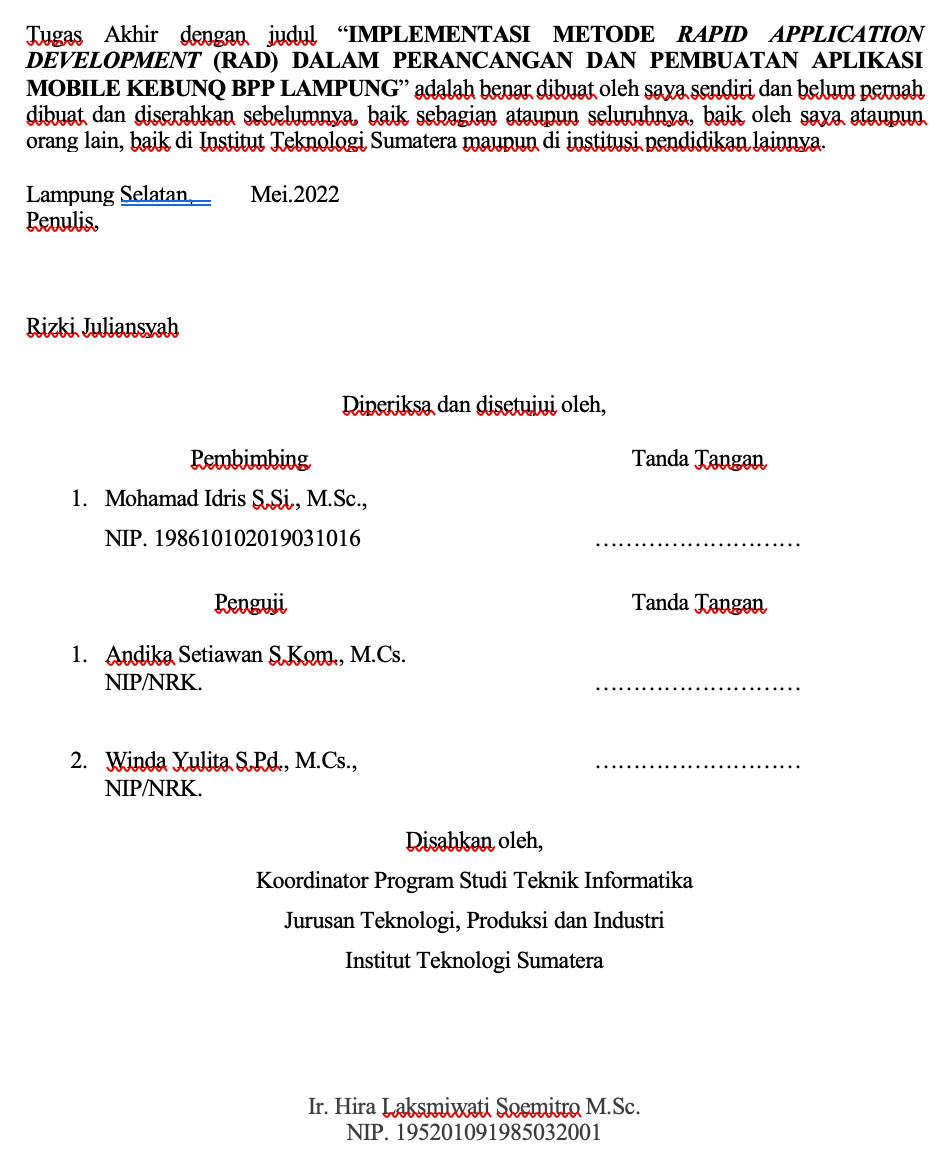
\includegraphics[width=15cm]{images/pengesahan.png}\\
                    
% % \renewcommand{\arraystretch}{0.5}
% \noindent Tugas Akhir dengan judul “Implementasi Metode \textit{Rapid Application Development} (RAD) Dalam Perancangan dan Pembuatan Aplikasi Mobile KebunQ BPP Lampung” adalah benar dibuat oleh saya sendiri dan belum pernah dibuat dan diserahkan sebelumnya, baik sebagian ataupun seluruhnya, baik oleh saya ataupun orang lain, baik di Institut Teknologi Sumatera maupun di institusi pendidikan lainnya.

% \noindent
% \vspace{0.2cm}
% \begin{tabularx}{\linewidth}{XX}
% \begin{minipage}{\linewidth}
% 	\noindent Lampung Selatan, \hspace{0.5cm} - \hspace{0.5cm}  - 2022
% \vspace{1.5cm}
% \noindent Penulis,\\
% Rizki Juliansyah\\
% NIM. 14116151
% \end{minipage} &
% \begin{minipage}{\linewidth}\centering

% Foto
% \end{minipage}
% \end{tabularx}

% \vspace{1cm}
% \onehalfspacing
% \centering\noindent Diperiksa dan disetujui oleh,

% \noindent
% \vspace{0.3cm}
% \begin{tabularx}{\linewidth}{XX}
% \begin{minipage}{\linewidth}
% 	\noindent Pembimbing\\
% % \vspace{2cm}
% \noindent 1. Mohamad Idris S.Si., M.Sc.,\\
% NIP. 198610102019031016
% \end{minipage} &
% \hspace{3cm}
% \begin{minipage}{\linewidth}
% 	\noindent Tanda Tangan\\
% 	% \vspace{2cm}
% 	\noindent \\
% 	.......................
% \end{minipage}
% \end{tabularx}

% \onehalfspacing
% \centering\noindent 

% \noindent
% \vspace{0.3cm}
% \begin{tabularx}{\linewidth}{XX}
% \begin{minipage}{\linewidth}
% 	\noindent Penguji\\
% % \vspace{2cm}
% \noindent 1. Andika Setiawan S.Kom., M.Cs.\\
% NRK. 19911127 2018 1 158\\\\
% \noindent 2. Winda Yulita S.Pd., M.Cs.,\\
% NIP. 
% \end{minipage} &
% \hspace{3cm}
% \begin{minipage}{\linewidth}
% 	\noindent Tanda Tangan\\
% % \vspace{2cm}
% \noindent \\
% ........................\\\\
% \noindent \\
% .......................
% \end{minipage}
% \end{tabularx}

% \vspace{2.5cm}
% \begin{center}
% \begin{minipage}{\linewidth}

% \vspace{1cm}
% Disahkan oleh, \\
% Koordinator Program Studi Teknik Informatika \\
% Jurusan Teknologi, Produksi dan Industri \\
% Institut Teknologi Sumatera\\
% \vspace{2.5cm}
% \underline{Kaprodi, S.Si, M.Si} \\
% NIP. XXXXXXX
% \end{minipage}
% \end{center}

\newpage
\onehalfspacing


% Lembar Pernyataan
\phantomsection \addcontentsline{toc}{chapter}{LEMBAR PERNYATAAN}
%
% Lembar pengesahan Naskah

\chapter*{\uppercase{HALAMAN PERNYATAAN ORISINALITAS}}
\centering
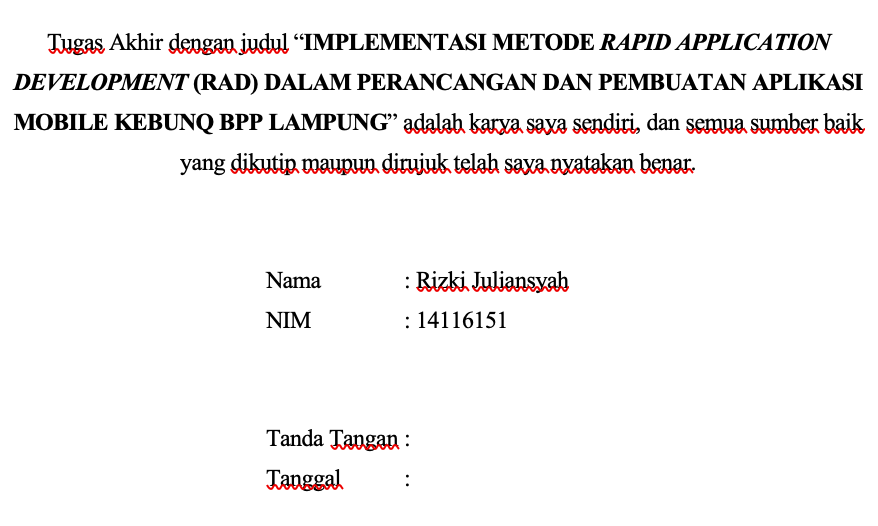
\includegraphics[width=14cm]{images/orisinal.png}\\
        
% \vspace{1cm}
% \noindent Tugas Akhir dengan judul “TULIS JUDUL DISINI” adalah karya saya sendiri, dan semua sumber baik yang dikutip maupun dirujuk telah saya nyatakan benar.

% \noindent Yang bertanda tangan di bawah ini:
% \renewcommand{\arraystretch}{1.5}
% \begin{table}[ht]
% \begin{adjustwidth}{-0.15cm}{}
% 	\begin{tabular}{lll}
% 		Nama & : & Rizki Juliansyah \\
% 		NIM & : & 14116151 \\
% 		Program Studi & : & Teknik Informatika \\
% 		Fakultas & : & Teknik \\
% 		Jenjang Pendidikan & : & Strata 1
% 	\end{tabular}
% \end{adjustwidth}
% \end{table} \\

% \vspace{-1cm}
% \noindent Menyatakan bahwa skripsi yang saya buat dengan judul:

% \vspace{0.3cm}
% \noindent PERANCANGAN SISTEM INFORMASI KOPERASI SIMPAN PINJAM BERBASIS WEB
% \begin{enumerate}[nolistsep,leftmargin=0.5cm]
% 	\item Merupakan hasil karya tulis ilmiah sendiri, bukan merupakan karya yang pernah diajukan untuk memperoleh gelar akademik oleh pihak lain, dan bukan merupakan hasil plagiat.
% 	\item Saya ijinkan untuk dikelola oleh Universitas Pamulang sesuai dengan norma dan etika yang berlaku.
% \end{enumerate}
% Pernyataan ini saya buat dengan penuh tanggung jawab dan saya bersedia menerima konsekuensi apapun sesuai aturan yang berlaku apabila dikemudian hari pernyataan ini tidak benar.

% \vspace{2cm}
% \begin{table}[ht]
% \begin{adjustwidth}{-0.15cm}{}
% 	\begin{tabular}{l}
% 	Pamulang, 01 Agustus 2014 \\[2cm]
% 	(Nama Orang)
% 	\end{tabular}
% \end{adjustwidth}	
% \end{table}

\newpage

% Lembar Persetujuan
\phantomsection \addcontentsline{toc}{chapter}{LEMBAR PERSETUJUAN}
%
% Lembar persetujuan
\doublespacing
\chapter*{\uppercase{LEMBAR PERSETUJUAN}}
\vspace{1cm}

\renewcommand{\arraystretch}{1.5}
\begin{table}[ht]
\begin{adjustwidth}{-0.15cm}{}
	\begin{tabularx}{\textwidth}{llX}
		Nama & : & Imron Rosdiadna \\
		NIM & : & 2010140419 \\
		Program Studi & : & Teknik Informatika \\
		Fakultas & : & Teknik \\
		Jenjang Pendidikan & : & Strata 1 \\
		Judul Skripsi & : & PERANCANGAN SISTEM INFORMASI KOPERASI SIMPAN PINJAM BERBASIS WEB
	\end{tabularx}
\end{adjustwidth}
\end{table}

\noindent Skripsi ini telah diperiksa dan disetujui. \\
Pamulang, 01 Agustus 2014

\vspace{3cm}
\begin{center}
\begin{minipage}{\linewidth}\centering
\underline{Pembimbing 1, S.Kom, M, Kom} \\
Pembimbing \\
\vspace{1cm}
Mengeetahui, \\
\vspace{3cm}
\underline{Kaprodi, S.Si, M.Si} \\
KaProdi Teknik Informatika
\end{minipage}
\end{center}

\newpage
\onehalfspacing

% Kata Pengantar
\phantomsection \addcontentsline{toc}{chapter}{KATA PENGANTAR}
% Kata Pengantar
\chapter*{KATA PENGANTAR}

% \blindtext \\[2cm]
\begin{justify}
\noindent Puji syukur kehadirat Allah SWT atas limpahan rahmat, karunia, serta petunjuk- Nya sehingga penyusunan tugas akhir ini telah terselesaikan dengan baik. Dalam penyusunan tugas akhir ini penulis telah banyak mendapatkan arahan, bantuan, serta dukungan dari berbagai pihak. Oleh karena itu pada kesempatan ini penulis mengucapan terima kasih kepada:
\end{justify}
\hfill
\begin{minipage}[t]{4.9cm}
\centering
	Pamulang, 01 Agustus 2014 \\ [2cm]
	Imron Rosdiana
\end{minipage}

\newpage

% Lembar Abstrak
\phantomsection \addcontentsline{toc}{chapter}{ABSTRAK}

\chapter*{ABSTRAK}
\noindent IMPLEMENTASI METODE \textit{RAPID APPLICATION DEVELOPMENT} (RAD) DALAM PERANCANGAN DAN PEMBUATAN APLIKASI MOBILE KEBUNQ BPP LAMPUNG\\
Rizki Juliansyah

\begin{singlespace}
    \begin{justify}
        
    Sektor pertanian merupakan sumber daya alam yang seharusnya dikelola dengan sebaik-baiknya. Urgensi pengoperasian teknologi yang efektif mempengaruhi produktivitas 
    pertanian, yaitu mempermudah pekerjaan petani sehingga memakan waktu yang tidak lama serta tidak dibutuhkannya lagi tenaga kerja manual.
    Balai Pelatihan Pertanian (BPP) Lampung juga masih mengharuskan tenaga kerja datang ke lokasi untuk melakukan \textit{monitoring} 
    dan kontrol kondisi lahan. Ketersediaan \emph{smartphone} di kalangan petani dapat memberikan dampak positif yaitu peningkatan produktivitas pertanian melalui
    penerapan Teknologi Informasi dan Komunikasi. Berdasarkan hal tersebut dilakukan perancangan dan pembuatan aplikasi KEBUNQ. 
    Perancangan dan pembuatan sebuah \emph{software} atau aplikasi tidak lepas dari 
    penerapan \emph{Software Development Life Cycle} (SDLC). SDLC bertujuan untuk memaksimalkan 
    output \emph{software} yang dibuat. Pada penelitian ini, SDLC yang digunakan adalah \emph{Rapid Application Development}
    (RAD). Pengujian yang dilakukan menggunakan metode \emph{black box testing} untuk menguji fungsionalitas aplikasi, dan \emph{User Acceptance Testing} (UAT) untuk mengetahui tingkat penerimaan pengguna. Pada penelitian ini, pengujian \emph{black box} didapatkan hasil yang sesuai dengan yang diharapkan. 
    Kemudian pada pengujian UAT, didapatkan hasil 85,77\% yang menunjukkan tingkat penerimaan yang sangat kuat oleh pengguna.\\[2cm]
        \textbf{Kata Kunci: \textit{Software Development Life Cycle, Smartphone, Rapid Application Development, Black box testing, User Acceptance Testing.}}
    \end{justify}

\end{singlespace}

\newpage

% Lembar Abstract
\phantomsection \addcontentsline{toc}{chapter}{ABSTRACT}
%
% Halaman Abstract

\chapter*{ABSTRACT}

\begin{singlespace}
\blindtext \\[20pt]
Keywords: \textit{Information System, Testing Project}
\end{singlespace}

\newpage





\vspace*{-2.5cm}
\tableofcontents
\phantomsection
\addcontentsline{toc}{chapter}{DAFTAR ISI}
\clearpage
\vspace*{-2.5cm}
\listoftables
\phantomsection
\addcontentsline{toc}{chapter}{DAFTAR TABEL}
\clearpage
\vspace*{-2.5cm}
\listoffigures
\phantomsection
\addcontentsline{toc}{chapter}{DAFTAR GAMBAR}
\clearpage

% KURANG DAFTAR LAMPIRAN

% Gunakan penomeran Arab (1, 2, 3, ...) setelah bagian ini.
\pagenumbering{arabic}

%
% Atur header dan footer dalam dokumen.
% 
\renewcommand{\headrulewidth}{0.0pt}
	\fancyhf{} 
	\fancyhead[L]{} 
	\fancyhead[C]{} 
	\fancyhead[R]{\thepage} 
	\renewcommand{\headrulewidth}{0.0pt}
	\renewcommand{\footrulewidth}{0.0pt} 
\pagestyle{fancy}

\onehalfspacing
%-----------------------------------------------------------------------------%

\chapter{PENDAHULUAN}
%-----------------------------------------------------------------------------%

\vspace{4.5pt}

\begin{flushleft}
  \begin{justify}
    \section{Latar Belakang} 
    Sektor pertanian merupakan sumber daya alam yang seharusnya dikelola dengan sebaik-baiknya. 
    Pengelolaan sektor pertanian yang baik dipengaruhi oleh penggunaan teknologi yang tepat guna dan keefektifan dalam pengoperasiannya. 
    Penggunaan teknologi yang tepat guna dipengaruhi oleh beberapa aspek lokal, diantaranya adalah aspek lingkungan, aspek sosial (sumber daya manusia lokal), dan aspek ekonomi masyarakat \cite{dokumenBalitbang,teknologi}. Namun, pengoperasian teknologi pada sektor pertanian beberapa diantaranya masih 
    memakan waktu yang lama dan menggunakan tenaga kerja manual. Urgensi pengoperasian teknologi yang efektif mempengaruhi produktivitas 
    pertanian, yaitu mempermudah pekerjaan petani sehingga memakan waktu yang tidak lama serta tidak dibutuhkannya lagi tenaga kerja manual. 

    Berdasarkan hasil wawancara terhadap penanggungjawab program smart farming BPP Lampung, menyatakan bahwa pengolahan lahan di 
    Balai Pelatihan Pertanian (BPP) Lampung mengharuskan tenaga kerja datang ke lokasi untuk melakukan \textit{monitoring} 
    kondisi lahan, diantaranya: pengecekan suhu udara, kelembapan udara, intensitas cahaya, suhu air, suhu tanah, ppm air, 
    pH tanah, pH air, kelembapan tanah, dan tekanan udara menggunakan alat pengukur. Selain \textit{monitoring}, dilakukan juga 
    kontrol sistem penyiraman pada lahan. Sistem \textit{monitoring} dan \textit{controlling} tersebut tergolong tidak efektif 
    dikarenakan masih beroperasi menggunakan tenaga kerja manual sehingga memakan waktu yang lama. Maka daripada itu diperlukannya  
    inovasi yang dapat mendukung keefektifan para petani dalam mengoperasikan teknologi. 

    \textit{Smartphone} merupakan teknologi yang berkembang pesat saat ini. Dalam referensi \cite{web-datasmartphone} 
    jumlah pengguna smartphone di Indonesia mencapai 170,4 juta. Jumlah petani per 2019 dalam catatan Badan Pusat Statistik (BPS) mencapai 33,4 juta orang \cite{databps}. 
    Jumlah petani di Indonesia akan terus bertambah mengingat perekonomian nasional sangat bergantung pada sektor pertanian sesuai dengan 
    referensi \cite{jurnal-kajianAplikasi} yang menyatakan bahwa 14,9\% dari Produk Domestik Bruto (PDB) berasal dari sektor pertanian. Berdasarkan data tersebut, ketersediaan \textit{smartphone} di kalangan petani Indonesia dapat memberikan dampak positif yaitu peningkatan produktivitas pertanian melalui penerapan Teknologi Informasi dan  Komunikasi (TIK). 

    Perancangan dan pembuatan sebuah \emph{software} atau aplikasi tidak lepas dari 
    penerapan \emph{Software Development Life Cycle} (SDLC). SDLC bertujuan untuk memaksimalkan 
    output \emph{software} yang dibuat, baik itu dari segi kualitas yang tinggi sesuai dengan ekspektasi 
    stakeholder dan para pengguna \cite{sdlc} dikarenakan SDLC berperan dalam perencanaan, 
    kontrol, transparansi, meminimalisir risiko, dan biaya dalam sebuah pengerjaan proyek \cite{sdlc2}. 
    Ada banyak jenis SDLC yang dapat diterapkan dengan menimbang kebutuhan dan keadaan pengembang, diantaranya \emph{waterfall} \cite{waterfall}, \emph{Agile} \cite{agile}, dan \emph{Rapid Application Development} (RAD) \cite{Sukamto}. Berdasarkan referensi \cite{Sukamto} RAD merupakan metode pengembangan yang cepat dikarenakan pengerjaan dapat dilakukan secara paralel oleh tim lain atau anggota lain dalam tim.

    Berdasarkan permasalahan di atas maka dilakukan penelitian pengembangan dengan judul \textbf{“Implementasi metode \textit{Rapid Application Development} (RAD) dalam perancangan dan pembuatan aplikasi \textit{mobile} KebunQ BPP Lampung”}.  Penelitian ini dilakukan sekaligus untuk membantu program \textit{Low Cost Smart Farming} BPP Lampung. Pemilihan metode RAD pada penelitian ini didasarkan atas ketersediaan waktu pengerjaan yang pendek \cite{Sukamto} dan jumlah tim pengembangan yang kecil \cite{jurnal empiris}.
\\

    \section{Rumusan Masalah}
      Berdasarkan latar belakang yang telah dipaparkan, maka rumusan masalahnya adalah sebagai berikut:
      \begin{enumerate}
        \item Bagaimana implementasi metode RAD dalam perancangan dan pembuatan aplikasi \textit{mobile} KEBUNQ?
        \item Bagaimana pengujian yang dilakukan pada aplikasi KEBUNQ?\\
      \end{enumerate}
    \section{Tujuan Penelitian}
      Adapun tujuan dalam penelitian ini adalah mengimplementasikan metode RAD dalam merancang dan membuat aplikasi \textit{mobile} KEBUNQ.
      \\
    \section{Batasan Masalah}
      Adapun batasan masalah dalam penelitian ini adalah sebagai berikut:
      \begin{enumerate}
        \item Penelitian perancangan dan pembuatan aplikasi KEBUNQ ini dibatasi pada pengoperasian aplikasi di sistem operasi android.
        \item Lahan yang diamati dan diimplementasikan aplikasi KEBUNQ dalam penelitian ini terbatas pada lahan cabai besar, lahan cabai kecil, dan \emph{screen} hidroponik di Balai Pelatihan Pertanian Lampung.\\
      \end{enumerate} 
    \section{Manfaat Penelitian}
    Penelitian ini diharapkan dapat bermanfaat bagi BPP Lampung dalam \textit{monitoring} dan \textit{controlling} pengelolaan lahan yang lebih efektif serta berguna dalam berjalannya program low cost smart farming BPP Lampung.
    \\


    \section{Sistematika Penulisan}
    Pada penelitian ini peneliti menyusun berdasarkan sistematika penulisan sebagai berikut: 
      \begin{itemize}
        \item BAB I PENDAHULUAN
        \\
        Bab ini berisi tentang latar belakang, rumusan masalah, tujuan penelitian, 
        batasan masalah, manfaat penelitian, dan sistematika penulisan.

        \item BAB II TINJAUAN PUSTAKA
        \\
          Bab ini berisi tentang teori-teori yang mendukung atau berhubungan dengan aplikasi ini.
        \item BAB III METODE PENELITIAN
        \\
          Bab ini berisi tentang teori-teori yang mendukung atau berhubungan dengan aplikasi ini.
        \item BAB IV HASIL IMPLEMENTASI DAN PEMBAHASAN
        \\
          Bab ini berisi tentang hasil implementasi dari rancangan penelitian beserta pembahasannya.
        \item BAB V KESIMPULAN DAN SARAN
        \\
          Bab ini berisi kesimpulan dan saran yang didapatkan dari penelitian ini.
        \\
      \end{itemize}

  \end{justify}

\end{flushleft}
\newpage
%-----------------------------------------------------------------------------%
\chapter{LANDASAN TEORI}
%-----------------------------------------------------------------------------%

%
\vspace{4.5pt}

\begin{flushleft}
    \section{Tinjauan Pustaka}
    \section{Dasar Teori}
    \begin{justify}
        \subsection{\textit{Monitoring} dan Kontrol}
        Menurut Dr. Harry Hikmat (2010), monitoring adalah proses pengumpulan
dan analisis informasi berdasarkan indikator yang ditetapkan secara sistematis dan
berkelanjutan tentang kegiatan/program sehingga dapat dilakukan tindakan
koreksi untuk penyempurnaan program/kegiatan itu selanjutnya
Sistem kontrol atau
sistem kendali adalah kumpulan dari beberapa komponen yang terhubung satu
sama lainnya, sehingga membentuk suatu tujuan tertentu yaitu mengendalikan
atau mengatur suatu sistem (Ogata, 1997). 
\\

        \subsection{Aplikasi \textit{Mobile}}
        Aplikasi \textit{mobile} adalah program perangkat lunak yang dirancang untuk dijalankan di smartphone, tablet, dan perangkat lain [N. Serrano]. Urgensi penggunaan Aplikasi yang dikembangkan berbasis mobile adalah semakin meningkatnya pengguna smartphone yang membutuhkan berbagai macam alat sebagai fasilitator dalam kegiatan sehari-hari. Sebagai fasilitator, aplikasi mobile harus mampu menyediakan informasi agar dapat menjadi sumber data bagi penggunanya dan mampu meningkatkan produktifitas pengguna. 
        \\
        \subsection{\textit{Rapid Application Development} (RAD)}
        Dalam referensi [\textbf{SUMBER}] terdapat lima tahapan dalam model RAD : (1) Pemodelan bisnis, (2) Pemodelan data, (3) Pemodelan proses, (4) Pembentukan aplikasi, (5) Pengujian dan \textit{turnover} .
        
        \begin{figure}[ht]
            \centering
           
	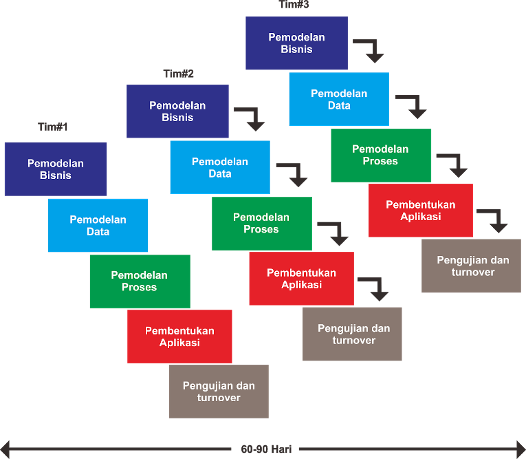
\includegraphics[width=6cm]{images/RAD.png}\\
            \caption{Gambar Ilustrasi Model RAD}
        \end{figure}
        Berdasarkan Gambar 3, dapat diperhatikan penjabaran sebagai berikut :
        \begin{enumerate}[label=\alph*.]
            \item Pemodelan Bisnis\\
            Pada tahap ini output yang dihasilkan berupa dokumen \textit{Software Requirements Specification} (SRS) yang meliputi informasi ketentuan aplikasi yang akan dibuat. Dokumen tersebut mencakup informasi apa saja yang harus dibuat, siapa yang harus membuat informasi itu, bagaimana alur informasi itu, proses apa saja yang terkait informasi itu.
            \item Pemodelan Data\\
            Memodelkan data apa saja yang dibutuhkan berdasarkan pemodelan bisnis dan mendefinisikan atribut-atributnya beserta relasinya dengan data-data yang lain. 
            \item Pemodelan Proses\\
            Mengimplementasikan fungsi bisnis yang sudah didefinisikan terkait dengan pendefinisian data. 
            \item Pembuatan Aplikasi\\
            Mengimplementasikan pemodelan proses dan data menjadi program. Model RAD sangat menganjurkan pemakaian komponen yang sudah ada jika dimungkinkan.
            \item Pengujian dan Pergantian\\
            Menguji komponen-komponen yang dibuat. Jika sudah teruji maka tim pengembang komponen dapat beranjak untuk mengembangkan komponen berikutnya.\\
        \end{enumerate}

        \subsection{Flutter}
        Flutter merupakan sebuah framework aplikasi mobile yang bersifat open source (terbuka) yang diciptakan oleh Google. Flutter dapat digunakan dalam pengembangan aplikasi mobile untuk sistem operasi Android dan iOS, bahkan juga dapat digunakan dalam pengembangan Web ataupun Desktop dari codebase tunggal. Flutter merupakan framework dengan penggunaan Bahasa Dart.
Berikut ini bebrapa kelebihan dari Flutter [\textbf{SUMBER}] :
\begin{enumerate}
    \item \textit{Package modules} sudah terkoneksi secara otomatis di dalam flutter, sehingga tidak terlalu repot untuk memanggil secara manual melalui terminal
    \item Dart menggunakan konsep OOP (\textit{Object Orinented Programming})
    \item \textit{Setup} secara manual jauh lebih mudah, apabila kita memerlukan \textit{library} baru, cukup tambahkan di bagian puspec.yaml
    \item Performa cepat dan  \textit{smooth}
    \item Data management menggunakan state sehingga lebih mudah dalam penggunaannya
    \item Adanya fitur \textit{Hot Reload} yang membantu debug lebih cepat
    \item Disupport oleh IDE yang sudah familiar dikalangan developer android, seperti Android Studio dan Visual Code\\
    
\end{enumerate}


        \subsection{\textit{Application Programming Interface} (API)}
            \textit{Application Programming Interface} atau API memungkinkan sebuah perusahaan untuk membuka data dan fungsionalitas aplikasi kepada \textit{developer} pihak ketiga / eksternal, mitra bisnis, dan departemen internal di dalam perusahaan tersebut. 
            Hal ini memungkinkan layanan dan produk untuk berkomunikasi satu sama lain dan memanfaatkan data dan fungsionalitas satu sama lain melalui \textit{interface} yang terdokumentasi. 
            \textit{Developer} tidak perlu tahu bagaimana API diimplementasikan; \textit{developer} hanya menggunakan \textit{interface} untuk berkomunikasi dengan produk dan layanan lain. 
            Penggunaan API telah melonjak selama dekade terakhir, sampai pada tingkat di mana banyak aplikasi web paling populer saat ini tidak akan mungkin tanpa API [\textbf{SUMBER}]. Secara tradisional, API merujuk ke \textit{interface} yang terhubung ke aplikasi yang mungkin telah dibuat dengan salah satu bahasa pemrograman tingkat rendah, seperti Javascript. API modern mematuhi prinsip REST dan format JSON dan biasanya dibuat untuk HTTP, menghasilkan \textit{interface} yang ramah kepada \textit{developer} yang mudah diakses dan dipahami secara luas oleh aplikasi yang ditulis dalam Java, Ruby, Python, dan banyak bahasa lainnya.
            \\


        \subsection{\textit{Database}}
        \textit{Database} adalah \textit{collection} dari informasi terstruktur yang terorganisir atau data, biasanya disimpan secara elektronik dalam sistem komputer [\textbf{SUMBER}]. Sebuah \textit{database} biasanya dikendalikan oleh \textit{Database Management System} (DBMS). Data dan DBMS bersama dengan aplikasi yang terkait dengannya disebut sebagai sistem basis data atau sering disingkat menjadi basis data saja.
        Data dalam tipe \textit{database} yang paling umum yang beroperasi saat ini biasanya dimodelkan sebagai baris dan kolom dalam serangkaian tabel untuk membuat pemrosesan dan kueri data menjadi efisien. Data kemudian dapat dengan mudah diakses, dikelola, dimodifikasi, diperbarui, dikendalikan, dan diatur. Sebagian besar \textit{database} menggunakan \textit{structured query language} (SQL) untuk menulis dan mengolah data. 
        Salah satu SQL yang sering digunakan adalah MySQL yang merupakan sistem manajemen basis data relasional yang tersedia \textit{open source} sehingga memudahkan pengguna.
        \\
        \subsection{\textit{Flowchart}}
        \textit{Flowchart} sering juga disebut dengan \textit{process flowchart, process flow diagram} atau diagram alir. Flowchart adalah gambaran langkah-langkah terpisah dari suatu proses secara berurutan. 
        \textit{Flowchart} sangat umum digunakan dan dapat diadaptasi untuk berbagai tujuan, dapat digunakan untuk menggambarkan berbagai proses, seperti proses manufaktur, proses administrasi/layanan, atau gambaran rencana proyek [\textbf{SUMBER}].
        Beberapa kondisi yang disarankan untuk menggunakan \textit{flowchart} yaitu 
        (1) Untuk membangun pemahaman tentang bagaimana suatu proses dilakukan,
        (2) Untuk mempelajari proses guna melakukan perbaikan,
        (3) Untuk mengomunikasikan kepada orang lain bagaimana suatu proses dilakukan,
        (4) Ketika komunikasi yang lebih baik diperlukan antara orang-orang yang terlibat dengan proses yang sama,
        (5) Untuk mendokumentasikan sebuah proses saat perencanaan proyek
        \\\\

        \subsection{\textit{Use Case} Diagram}

        \subsection{\textit{Black Box Testing}}

        \subsection{\textit{User Acceptance Testing} (UAT)}
        \noindent User Acceptance Testing (UAT) adalah pengujian terakhir yang dilakukan oleh user secara langsung, dan pada saat pengujian berlangsung pembuatan dokumen juga dilakukan sebagai bukti penerimaan sistem oleh pengguna. 
        \textcolor{red}{[Mutiara, A. B., Awaludin, R., Muslim, A. and T. Oswari, “Testing Implementasi Website Rekam Medis Elektronik Opeltgunasys Dengan Metode Acceptance Testing,” 2014.].
        }
        

        \subsection{Skala \textit{Likert}}

    \end{justify}



\end{flushleft}



\newpage
%-----------------------------------------------------------------------------%
\chapter{METODE PENELITIAN}
%-----------------------------------------------------------------------------%

%
\vspace{4.5pt}

\begin{flushleft}
   \begin{justify}
      \section{Alur Penelitian}

   \section{Penjabaran Langkah Penelitian}
    Berikut ini merupakan prosedur penelitian yang dilakukan mengikuti ilustrasi model RAD.
   \subsection{Studi Literatur}
 Mencari dan mengumpulkan referensi yang berkaitan dengan penelitian melalui media buku, jurnal dan e-book.
      
\subsection{Observasi}
Melakukan pengamatan di Balai Pelatihan Pertanian (BPP) Lampung terkait sistem pengolahan lahan cabai dan greenhouse.
   \section{Alat dan Bahan Tugas Akhir}
   \subsection{Alat}
   \subsection{Bahan}
   \end{justify}
   
\end{flushleft}

\vspace{5cm}
\noindent \textbf{CONTOH Penulisan}
\section{Analisa Sistem}

\subsection{Analisa Sistem Saat Ini}
Analisa sistem pendukung keputusan dalam penentuan penjurusan dibuat oleh peneliti dalam bentuk use case diagram yang mewakili secara sederhana dan bisa dijadikan sebagai bahan dalam evaluasi sistem yang berjalan, sehingga sistem dapat terlihat tanpa harus mengetahui secara detail prosedur yang berjalan.
\begin{figure}[ht]
	\centering
	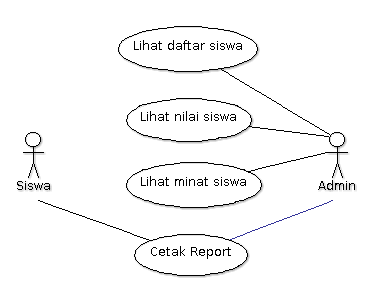
\includegraphics[width=10cm]{images/UseCaseDiagramSistemSaatIni}
	\caption{Use Case Diagram Analisa Sistem Saat Ini}
\end{figure}

\newpage
\noindent Dibawah ini merupakan deskripsi dari use case yang sedang berjalan:
\begin{enumerate}[nolistsep,leftmargin=0.5cm]
\item \textit{Admin} melihat daftar siswa.
\item \textit{Admin} melihat nilai setiap siswa.
\item \textit{Admin} melihat minat setiap siswa.
\item \textit{Admin} mencetak hasil keputusan.
\item Siswa melihat laporan penjurusan yang telah dicetak oleh \textit{admin}
\end{enumerate}

\subsection{Evaluasi Sistem Saat Ini}

\begin{table}[ht]
\centering
\caption{Permasalahan dan Solusinya}
\begin{tabular}{|>{\raggedright}p{5cm}|p{2.5cm}|>{\raggedright}p{5cm}|}
 \hline
 \multicolumn{1}{|c}{\bfseries Masalah} & \multicolumn{1}{|c|}{\bfseries Aktor} & \multicolumn{1}{c|}{\bfseries Solusi} \\ 
  \hline
\begin{enumerate}
   	\item Masalah masalah masalah Masalah masalah masalah Masalah masalah masalah Masalah masalah masalah.
   	\item Masalah masalah masalah Masalah masalah masalah Masalah masalah masalah Masalah masalah masalah.
   	\item Masalah masalah masalah Masalah masalah masalah Masalah masalah masalah Masalah masalah masalah.
   \end{enumerate} &
   \begin{enumerate}
  	\item Aktor 1
  	\item Aktor 2
  \end{enumerate} &
  \begin{enumerate}
  \item Solusi solusi solusi Solusi solusi solusi Solusi solusi solusi Solusi solusi solusi Solusi solusi solusi.
  \item Solusi solusi solusi Solusi solusi solusi Solusi solusi solusi Solusi solusi solusi Solusi solusi solusi.
  \item Solusi solusi solusi Solusi solusi solusi Solusi solusi solusi Solusi solusi solusi Solusi solusi solusi.
  \end{enumerate}
     \tabularnewline
  \hline
 \end{tabular}
\end{table}

\subsection{Model yang Diusulkan}

\subsection{Acitivity Diagram yang Diusulkan}

\subsection{Perancangan Prosedur Sistem}

\subsubsection{Use Case Diagram}

\subsubsection{Activity Diagram}
\begin{enumerate}[nolistsep,leftmargin=0.5cm]
\item \textit{Activity diagram} satu

\begin{enumerate}[label=\alph*.]
	\item Item 1.
	\item Item 2.
	\end{enumerate}
\item Dua
\end{enumerate}

\subsubsection{Class Diagram}

\subsubsection{Sequence Diagram}

\subsection{Perancangan Antarmuka (Interface)}

\newpage
%-----------------------------------------------------------------------------%
\chapter{HASIL PENELITIAN DAN PEMBAHASAN}
%-----------------------------------------------------------------------------%

%
\vspace{4.5pt}
\begin{flushleft}
    \begin{justify}
        \section{Hasil Penelitian}
        \subsection{Hasil Observasi}
        Peneliti mengamati kebutuhan sensor dan kontrol yang sering diaplikasikan pada lahan untuk kebutuhan pembuatan aplikasi KEBUNQ. Didapat data sebagai berikut.\\
        \subsubsection{Sensor} 
        Berikut beberapa sensor yang biasa digunakan pada lahan pertanian yang perlu dicantumkan ke aplikasi KEBUNQ :
        \begin{enumerate}
            \item Suhu
            \item \emph{Humidity}
            \item Intensitas Cahaya
            \item Suhu Tanah
            \item \emph{Humidity} Tanah
            \item pH Tanah
            \item Suhu Air
            \item TDS (ppm meter)
            \item pH Air\\
        \end{enumerate}
        \subsubsection{Kontrol}
        Berikut beberapa kontrol yang biasa digunakan pada lahan pertanian yang perlu dicantumkan ke aplikasi KEBUNQ :
        \begin{enumerate}
            \item \emph{Mist} 
            \item \emph{Sprinkler} 
            \item \emph{Fan} 
            \item \emph{Valve} 
            \item \emph{Drip} 
            \item Pompa 
            \item Lainnya (\emph{Customize})\\
        \end{enumerate}
        % \caption{Gambar Observasi}
        \subsection{Hasil Penerapan RAD}
        \subsubsection{Pemodelan Bisnis}
        Berdasarkan hasil analisa ditentukan bahwa aplikasi KEBUNQ dirancang untuk satu jenis pengguna. Sehingga tidak terdapat level pengguna pada akses aplikasi.
        Berikut analisa kebutuhan pengguna
        \begin{enumerate}
            \item Pengguna harus melakukan login
            \item Pengguna dapat melihat daftar dan status nyala alat
            \item Pengguna dapat melihat detail alat yang terdiri dari data sensor dan kontrol yang tersedia
            \item Pengguna dapat melakukan kontrol pada alat yang dipilih
            \item Pengguna dapat melakukan setting automatis pada suatu kontrol yang tersedia mode automatisnya\\
        \end{enumerate}
       
        \subsubsection{Pemodelan Data}
        \begin{figure}[ht]
            \centering
            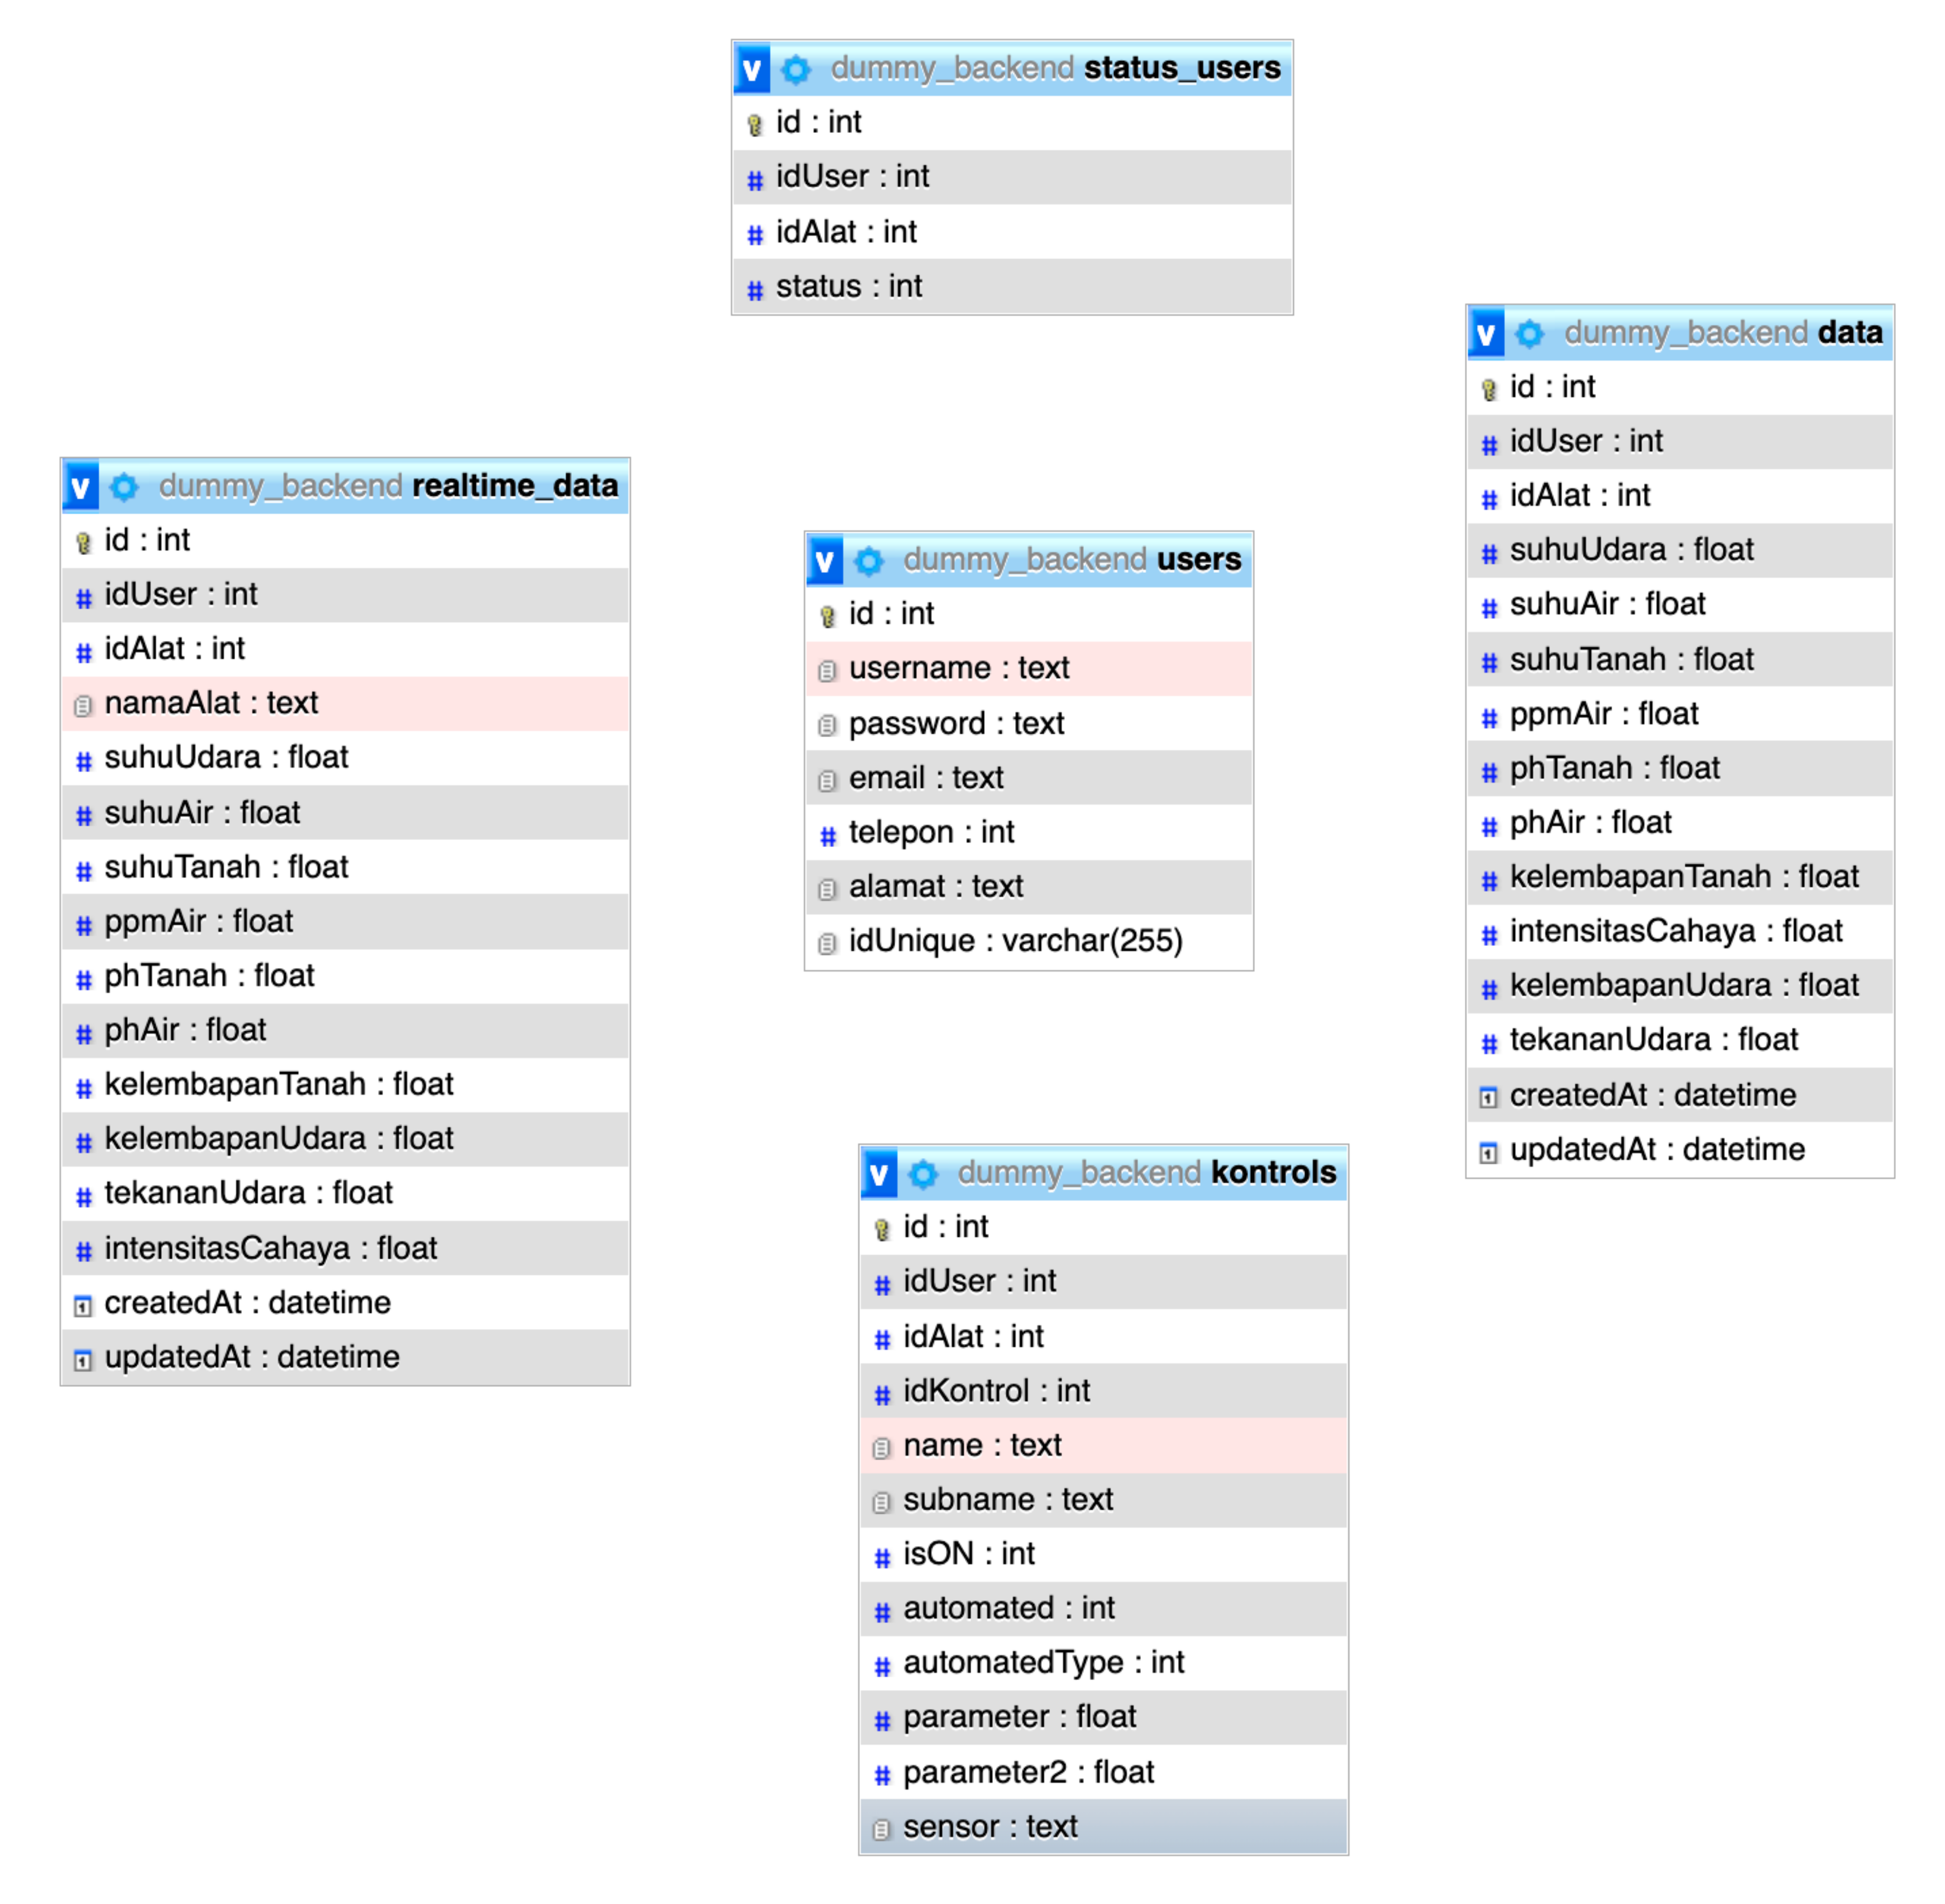
\includegraphics[width=8cm]{images/database.png}
            \caption{Skema Tabel \textit{Database}}
        \end{figure}
        \noindent \\Setelah dilakukan tahap pemodelan bisnis, maka didapatkan skema \emph{database} yang dirancang seperti gambar 4.1 di atas. \emph{Database} terdiri dari lima tabel yakni (1) tabel data, digunakan untuk menyimpan data time series dari nilai sensor yang ada pada alat, 
        (2) tabel kontrols, digunakan untuk menyimpan dan mendefinisikan kontrol yang dimiliki, 
        (3) tabel realtime\_data, digunakan untuk menyimpan data realtime sensor dan kontrol,
        (4) tabel status\_users, digunakan untuk menyimpan status alat apakah \emph{online} atau \emph{offline},
        dan (5) tabel users, digunakan untuk menyimpan data user. Setelah skema \emph{database} difinalisasi, 
        maka dilakukan pembuatan \emph{Application Programming Interface} (API) dan konfigurasi server yang dalam bagian ini 
        pengerjaan bukan dilakukan oleh peneliti namun oleh anggota lain dalam proyek. 
        Sehingga akhirnya didapat beberapa API (\emph{dummy}) sebagai berikut dengan \emph{endpoint} yang dirahasiakan demi keamanan aplikasi :
            \begin{itemize}
                \item API login\\
                http://47.89.212.89/dummyBackend/(\emph{endpoint})
                \item API \emph{Summary Data} dari pengguna\\
                http://47.89.212.89/dummyBackend/data/(\emph{endpoint})
                \item API data \emph{realtime}\\
                http://47.89.212.89/dummyBackend/data/mobile/(\emph{endpoint})
                \item API data kontrol\\
                http://47.89.212.89/dummyBackend/kontrol/(\emph{endpoint})
                \item API data ikon\\
                http://47.89.212.89/dummyBackend/(\emph{endpoint}) \\
                (\emph{endpoint} berada pada API data \emph{realtime})
                \item API status alat\\
                http://47.89.212.89/dummyBackend/status/(\emph{endpoint})
                \item API update kontrol\\
                http://47.89.212.89/dummyBackend/kontrol/(\emph{endpoint})
            \end{itemize}
        API ini digunakan oleh peneliti dalam tahap pembuatan aplikasi \emph{mobile} KEBUNQ sebagai penghubung antara aplikasi dengan \emph{database server}.\\
        

        

        \subsubsection{Pemodelan Proses}
        \begin{enumerate}[label=\alph*.]
            \item \textit{Use Case}
            \textit{Use case} perancangan aplikasi mobile KEBUNQ BPP Lampung yang dirancang setelah menganalisa tahap pemodelan bisnis dan 
            pemodelan data dapat dilihat pada Gambar 4.2
            \begin{figure}[ht]
                \centering
                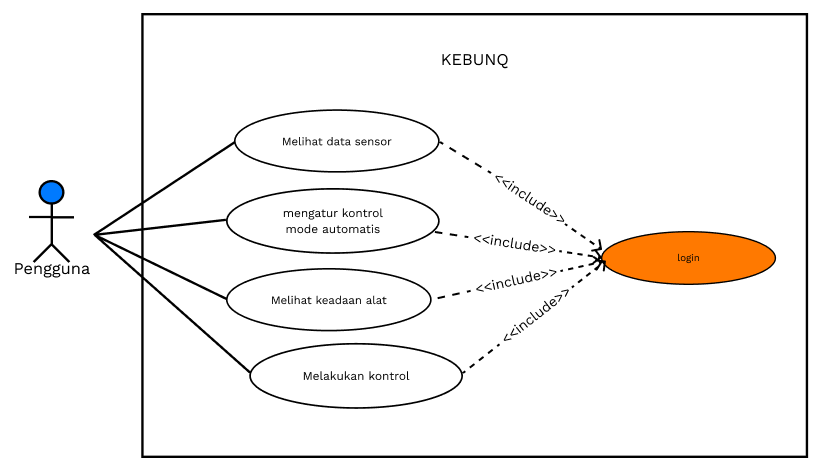
\includegraphics[width=10cm]{images/bab 4/use-case-user.png}
                \caption{\textit{Use Case Diagram}}
            \end{figure}
            \item \textit{Sequence Diagram}
            \begin{figure}[ht]
                \centering
                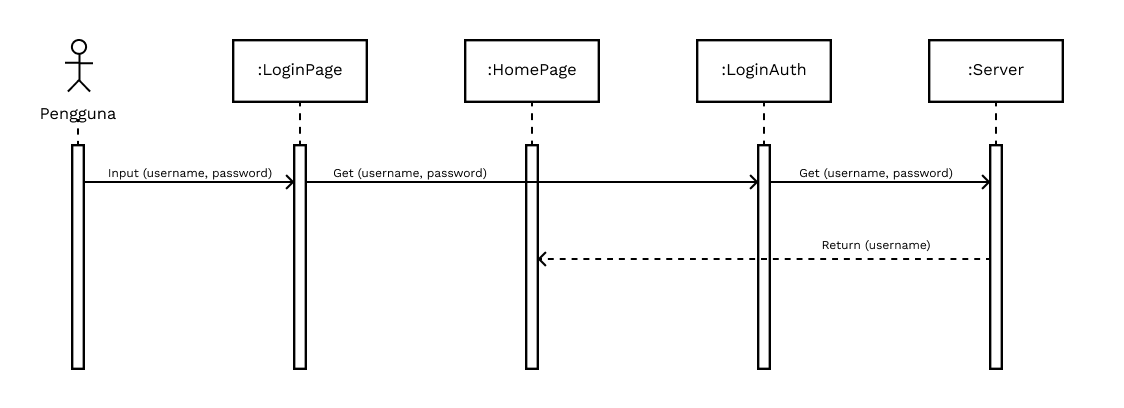
\includegraphics[width=12cm]{images/bab 4/Sequence login.png}
                \caption{\textit{Sequence Diagram Login}}
            \end{figure}
            \begin{figure}[ht]
                \centering
                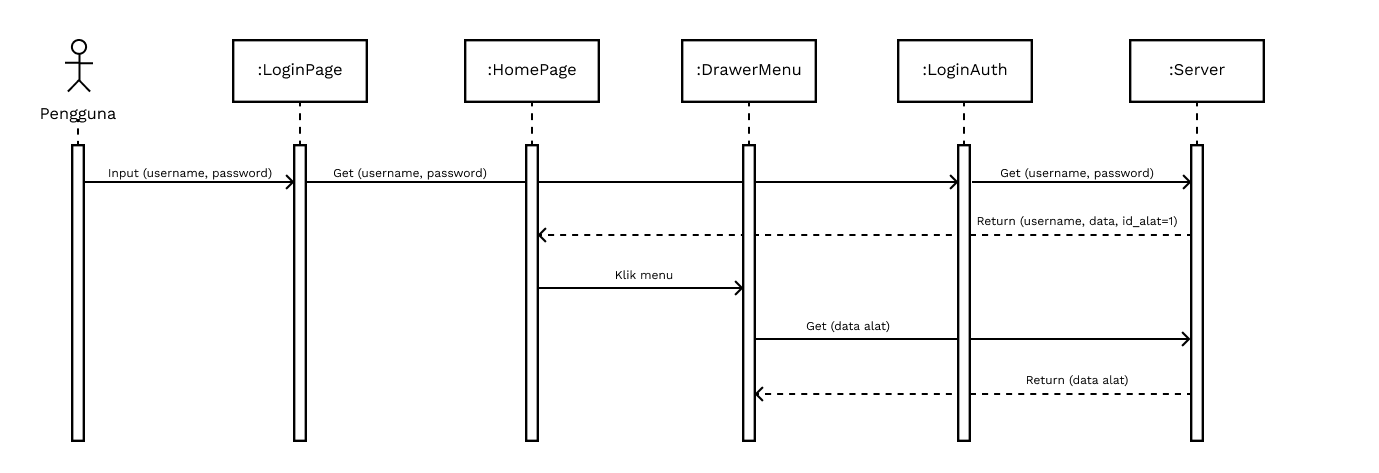
\includegraphics[width=12cm]{images/bab 4/buka menu alat.png}
                \caption{\textit{Sequence Diagram} Melihat Menu / Alat}
            \end{figure}
            \vspace{5cm}
            \begin{figure}[ht]
                \centering
                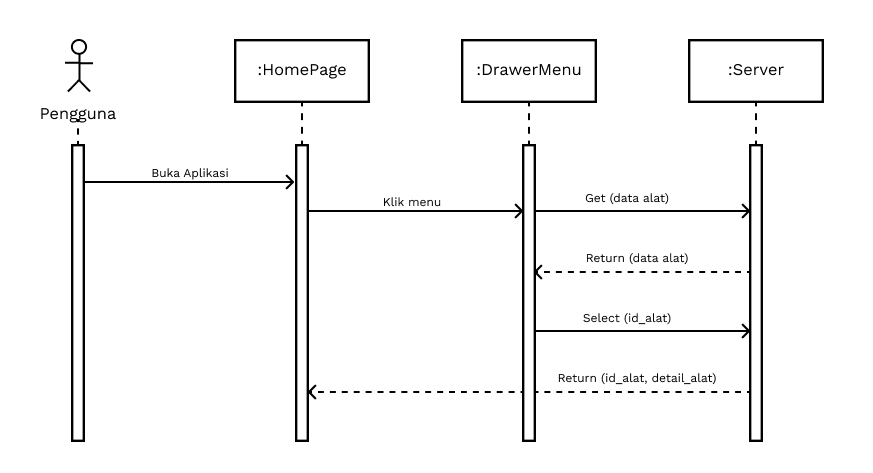
\includegraphics[width=14cm]{images/bab 4/Sequence buka detail alat.png}
                \caption{\textit{Sequence Diagram} Melihat Detail Alat}
            \end{figure}

            \begin{figure}[ht]
                \centering
                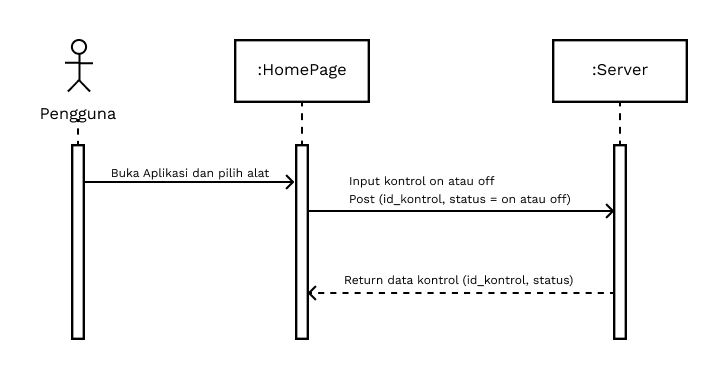
\includegraphics[width=14cm]{images/bab 4/Sequence kontrol.png}
                \caption{\textit{Sequence Diagram} Melakukan Kontrol}
            \end{figure}
            \begin{figure}[ht]
                \centering
                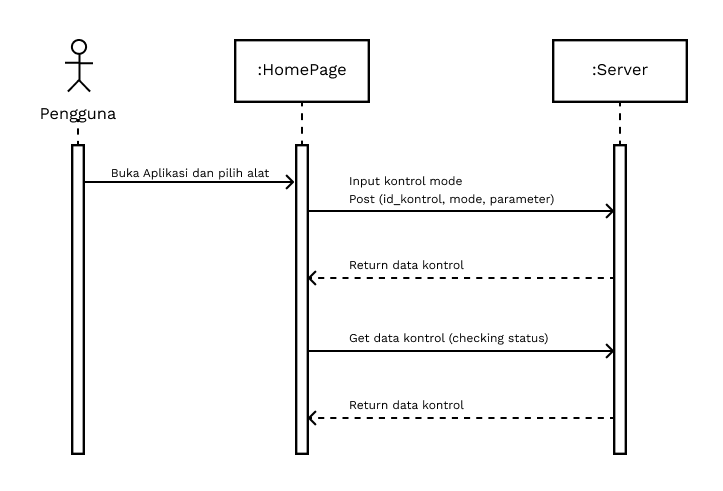
\includegraphics[width=11cm]{images/bab 4/Sequence kontrol Auto.png}
                \caption{\textit{Sequence Diagram} Melakukan Kontrol Automatis}
            \end{figure}
            \end{enumerate}
            \noindent \\\\\\\\\\\\\\\\
        \subsubsection{Pembuatan Aplikasi}
        Dalam proses pembuatan aplikasi peneliti melakukan 3 pengerjaan (1) Perancangan desain layout \textit{User Interface}, (2) Pembuatan \textit{assets} mencakup logo aplikasi, ikon sensor, dan ilustrasi kontrol, dan (3) Pengerjaan pembuatan aplikasi menggunakan \textit{framework} Flutter dengan bahasa pemrograman Dart
        \begin{enumerate}
            \item Perancangan Desain Layout \textit{User Interface}
            \begin{figure}[ht]
                \centering
                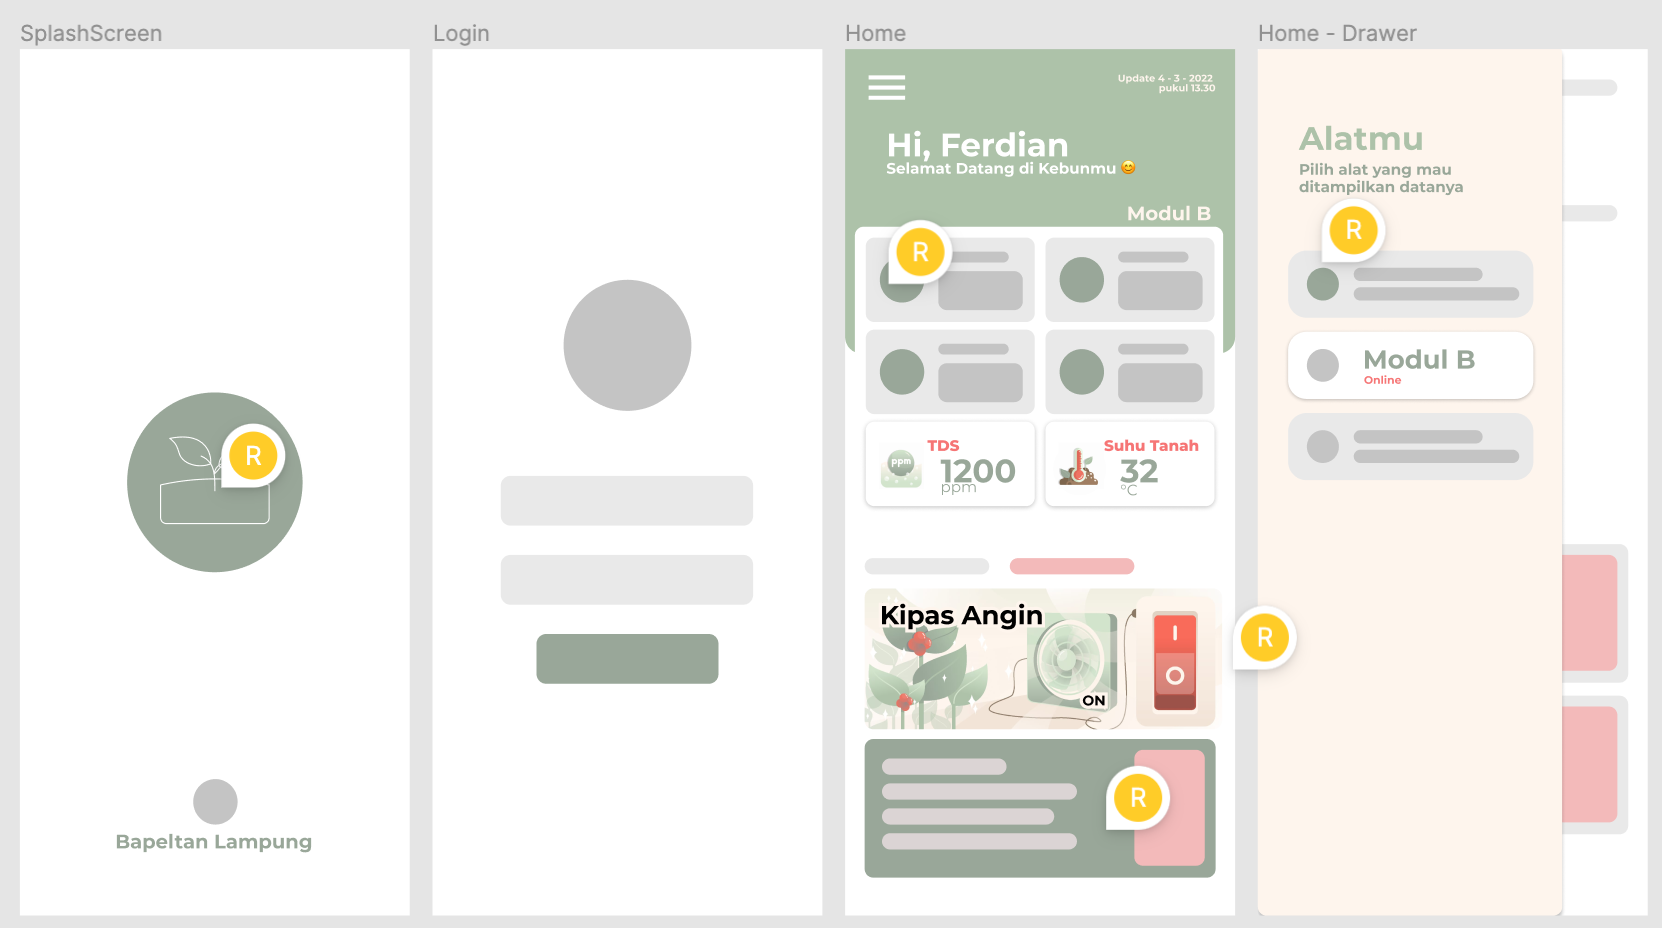
\includegraphics[width=15cm]{images/UI/summary.png}
                \caption{Rancangan layout UI}
            \end{figure}
            \vspace{10cm}
            \item Pembuatan \textit{assets}\\
            \begin{figure}[ht]
                \centering
                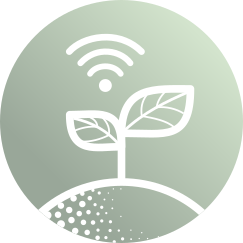
\includegraphics[width=6cm]{images/logo.png}
                \caption{\textit{assets} Logo aplikasi}
            \end{figure}
            \noindent \\Logo aplikasi KEBUNQ yang dirancang memiliki arti sebagai berikut :
            \begin{itemize}
                \item Bentuk koin : menunjukkan bahwa aplikasi KEBUNQ dirancang untuk mendukung program \emph{low cost smart farming}
                \item Tanda sinyal : menunjukkan penggunaan aplikasi memerlukan konektivitas jaringan internet untuk melakukan pemantauan dan kontrol dari jarak jauh (\emph{online apps})
                \item Tanaman : menunjukkan bahwa aplikasi KEBUNQ berhubungan erat dan tidak lepas dengan tanaman dalam penggunaannya
                \item pijakan tanaman dan bulatan-bulatan kecil : mewakilkan banyaknya unsur yang dapat kita pantau melalui aplikasi KEBUNQ.\\\\
            \end{itemize}
            \begin{figure}[ht]
                \centering
                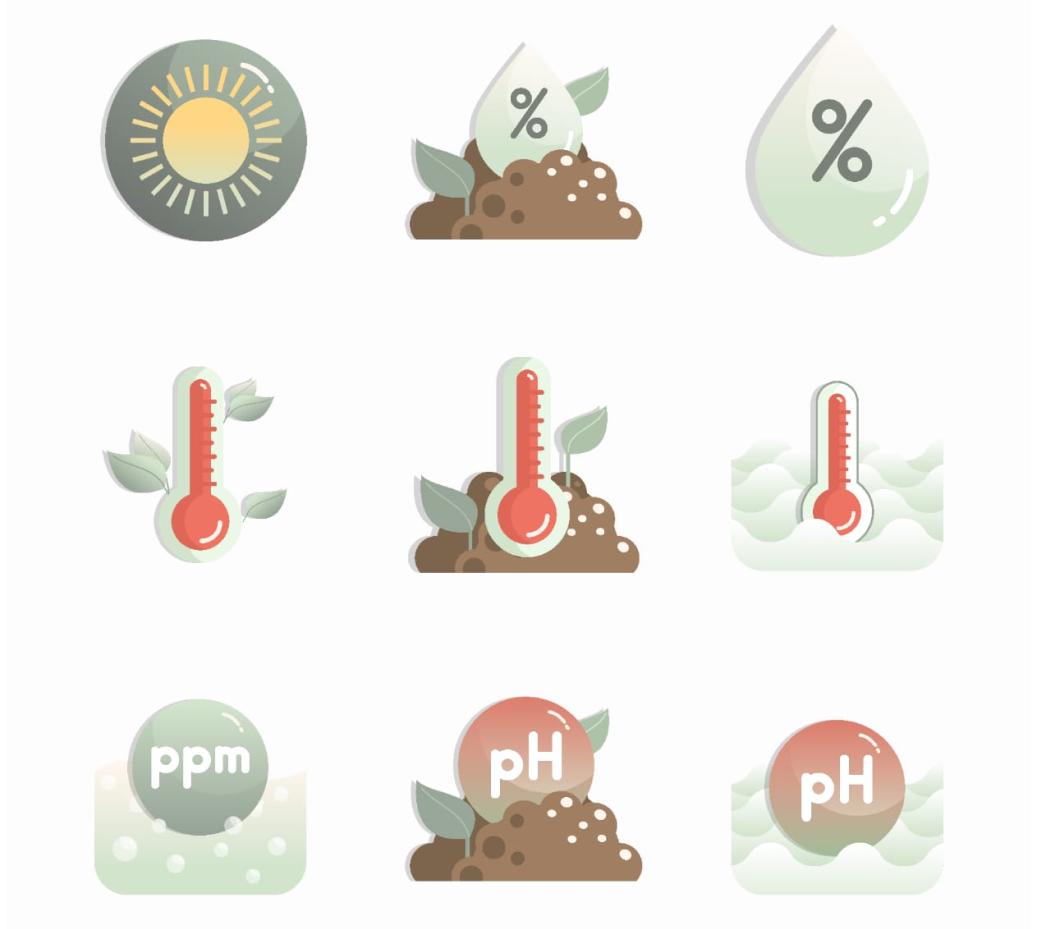
\includegraphics[width=7cm]{images/UI/ikon.png}
                \caption{\textit{assets} Ikon Sensor}
            \end{figure}
            \begin{figure}[ht]
                \centering
                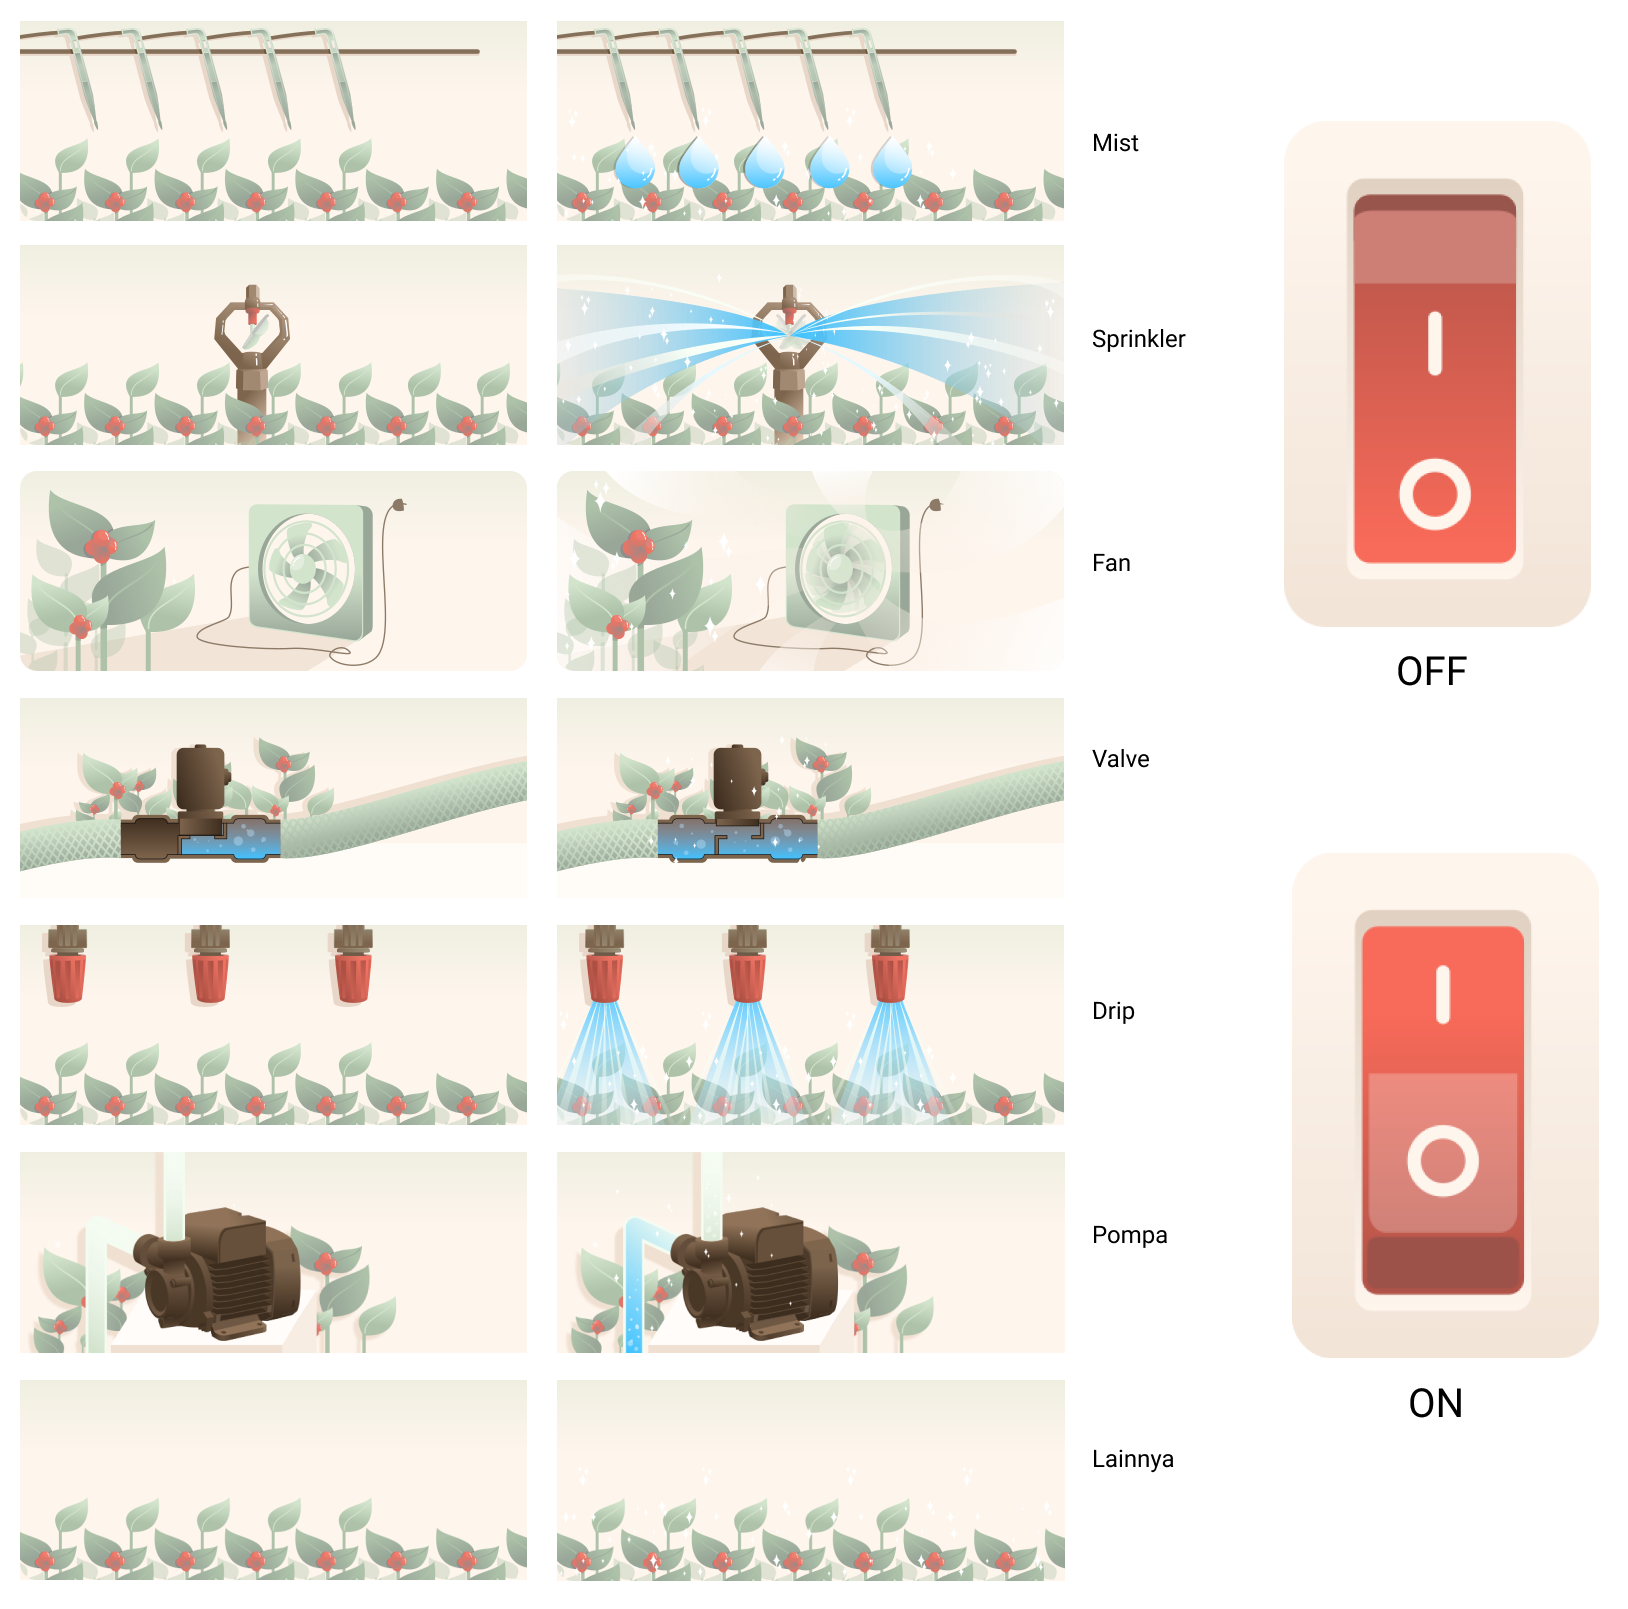
\includegraphics[width=7cm]{images/UI/Frame 1.png}
                \caption{\textit{assets} Kontrol}
            \end{figure}
            \noindent \\\\\\\\\\\\\\\\\\Pembuatan \emph{assets} logo, ikon dan ilustrasi bertujuan untuk meningkatkan kemudahan pengguna dalam menggunakan aplikasi KEBUNQ dan menjadikan KEBUNQ sebagai aplikasi yang unik dengan menggunakan \emph{assets} yang orisinil khusus didesain dan digunakan pada aplikasi KEBUNQ. \\
            \item Pembuatan Aplikasi\\
            Implementasi dari perancangan aplikasi KEBUNQ
            \begin{itemize}
                \item Halaman \emph{Splash Screen}\\
                Merupakan halaman pertama yang dilihat dengan hitungan waktu beberapa detik. Pada aplikasi KEBUNQ, \emph{splash screen} dibuat dengan sedikit implementasi gerak animasi dan mencantumkan logo KEBUNQ dan BPP Lampung.
                Halaman \emph{Splash Screen} dapat dilihat pada Gambar 4.12
                \begin{figure}[ht]
                    \centering
                    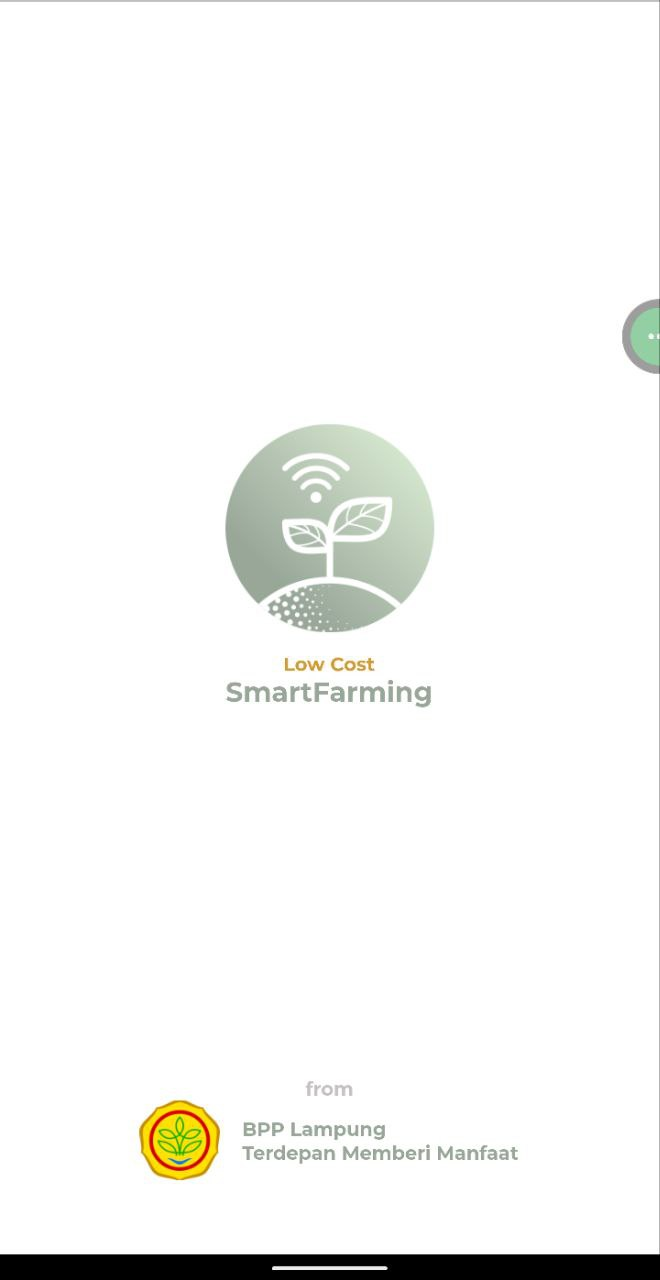
\includegraphics[width=3cm]{images/bab 4/splash.jpeg}
                    \caption{Tampilan \emph{Splash Screen}}
                \end{figure}

                \item Halaman \emph{Login}\\
                Halaman \emph{login} berupa formulir \emph{login} yang diharuskan untuk diisi dengan benar supaya kemudian pengguna dapat menggunakan fitur utama aplikasi KEBUNQ. Halaman login menampilkan \emph{field username} dan \emph{password}.
                Dalam proses \emph{login} dilakukan pemeriksaan data apakah data yang dimasukkan sesuai dengan \emph{database} atau tidak. Jika ada maka aplikasi KEBUNQ akan menampilkan halaman \emph{Home} dan menampilkan data yang dimiliki oleh pengguna. \
                Halaman \emph{login} dapat dilihat pada Gambar 4.13
                \begin{figure}[ht]
                    \centering
                    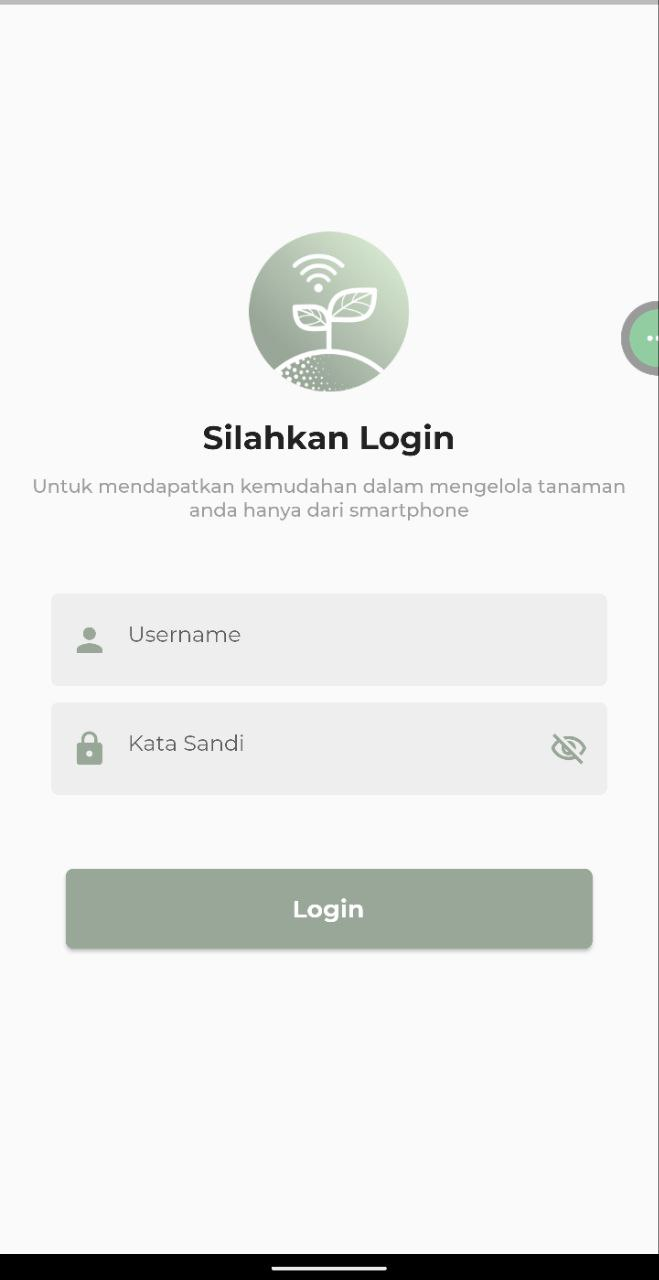
\includegraphics[width=3cm]{images/bab 4/login.jpeg}
                    \caption{Tampilan Halaman \emph{Login}}
                \end{figure}
                \vspace{10cm}
                \item Halaman \emph{Home}\\
                Halaman \emph{Home} merupakan halaman utama yang digunakan pengguna untuk melihat data sensor dan kontrol yang ada. Pengguna dapat melakukan kontrol atau kendali dengan cara menyalakan atau mematikan kontrol maupun memberikan \emph{setting} automatis pada kontrol yang dipilih.
                Halaman \emph{Home} dapat dilihat pada Gambar 4.14
                \begin{figure}[ht]
                    \centering
                    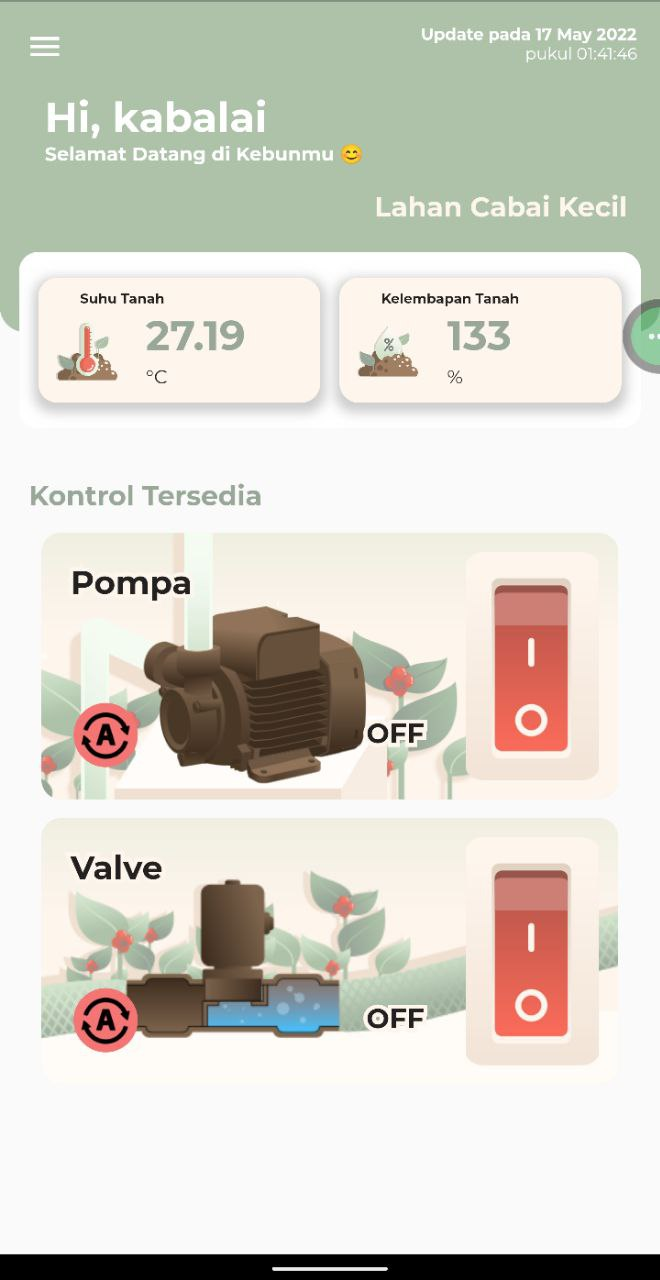
\includegraphics[width=3cm]{images/bab 4/home.jpeg}
                    \caption{Tampilan Halaman \emph{Home}}
                \end{figure}
                \newline
                \item \emph{Drawer}\\
                \emph{Drawer} merupakan bagian tampilan Menu yang terdapat pada halaman \emph{Home} ketika diklik/disentuh. Menu \emph{drawer} berisikan \emph{list} alat yang tersedia pada akun pengguna. Pada \emph{list} alat tersebut terdapat nama alat dan status keadaan alat sekarang apakah \emph{online} (keadaan nyala) atau \emph{offline} (keadaan mati).
                Tampilan menu \emph{drawer} dapat dilihat pada Gambar 4.15
                \begin{figure}[ht]
                    \centering
                    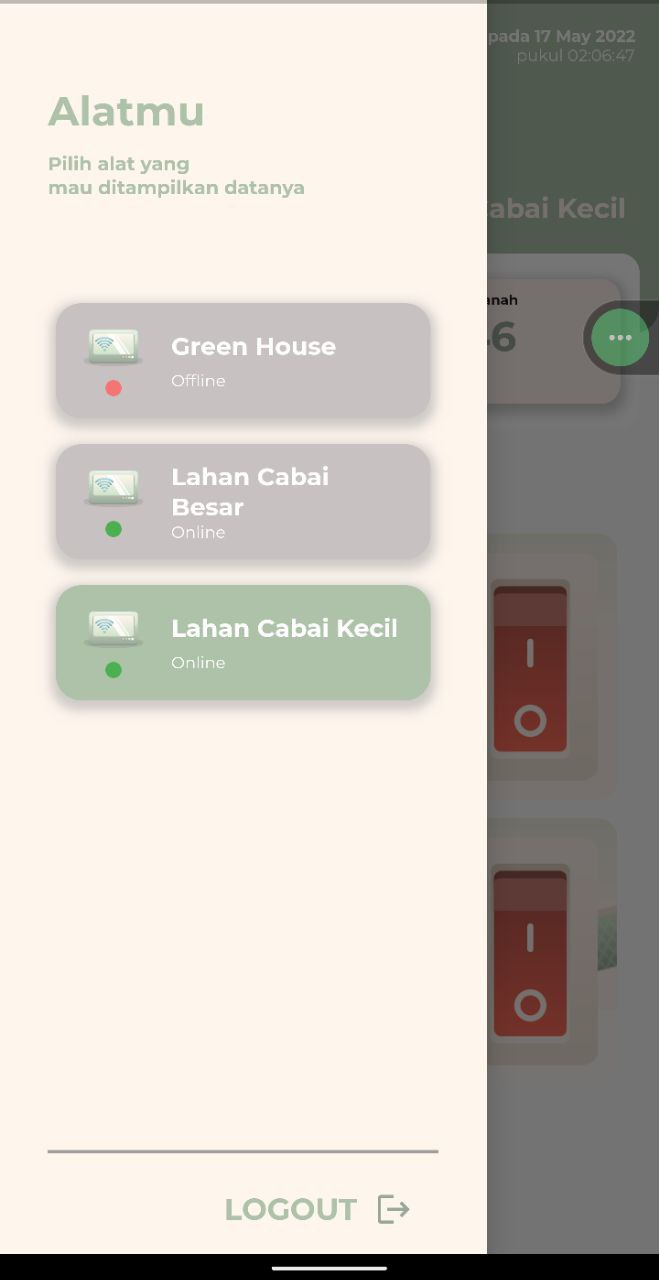
\includegraphics[width=3cm]{images/bab 4/drawerr.jpeg}
                    \caption{Tampilan Menu \emph{Drawer}}
                \end{figure}
                \item Tampilan \emph{Loading}
                Tampilan \emph{loading} merupakan tampilan yang muncul membentuk \emph{shimmer} pada layout yang dibuat ketika aplikasi KEBUNQ menunggu \emph{loading request} data dari API.
                Tampilan \emph{loading} dapat dilihat pada Gambar 4.16 
                \begin{figure}[ht]
                    \centering
                    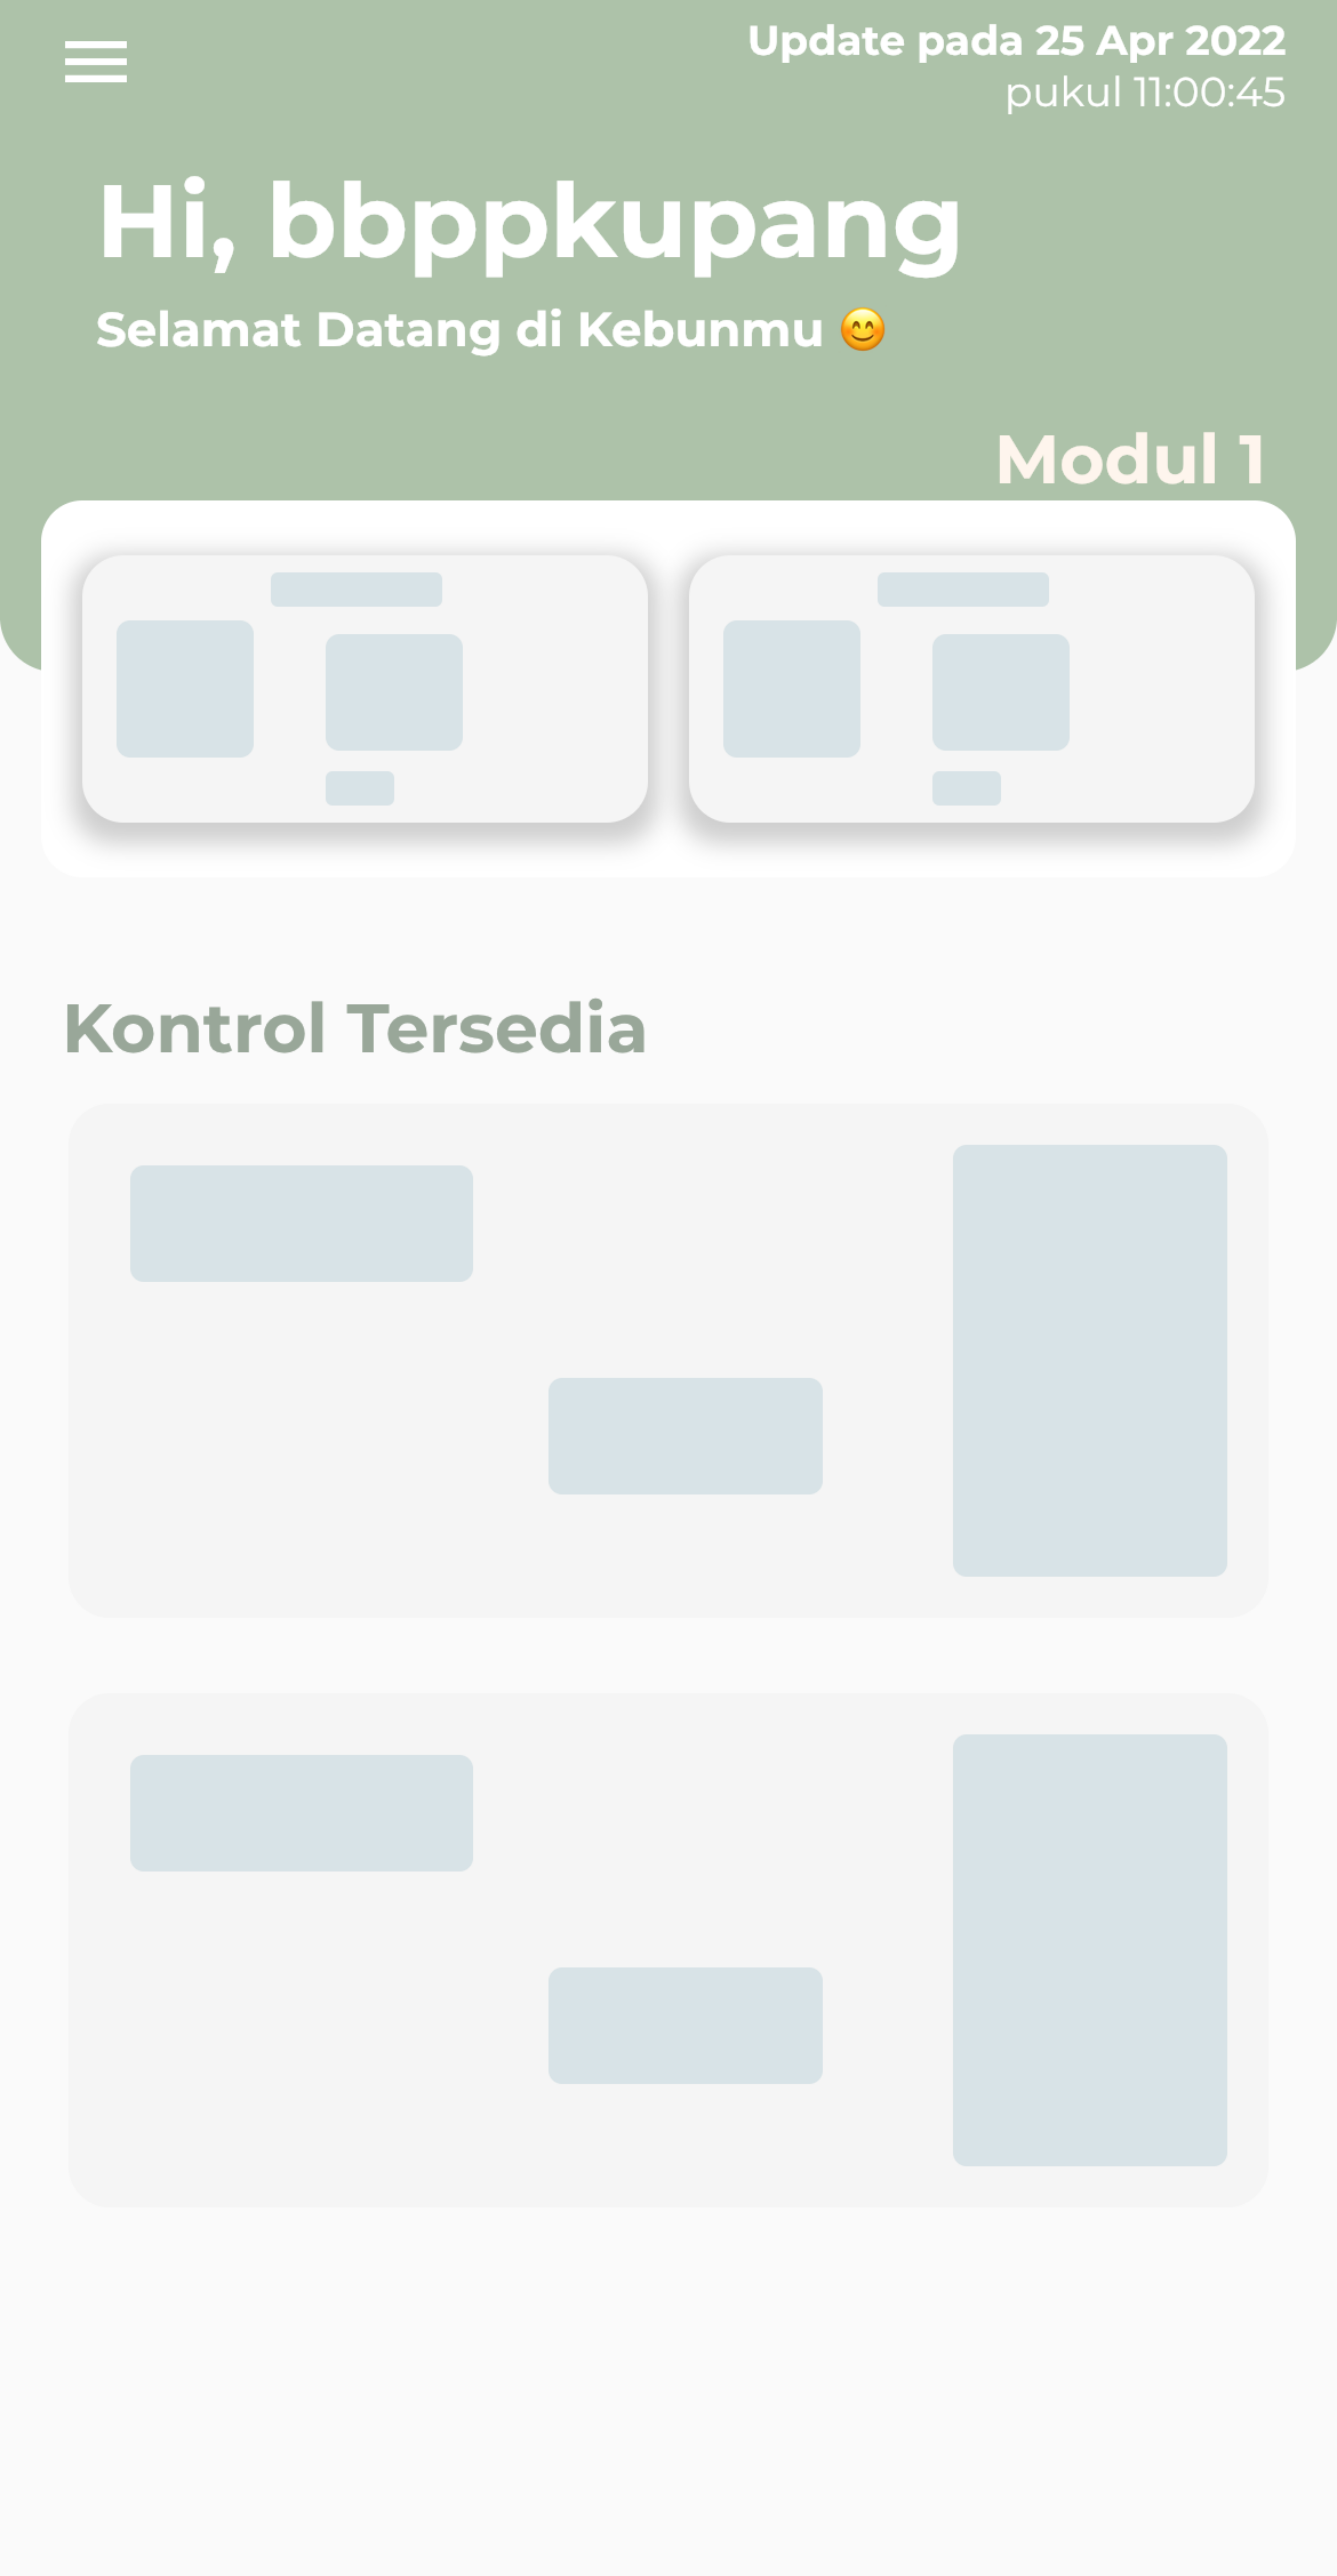
\includegraphics[width=3cm]{images/bab 4/ui-loading.png}
                    \caption{Tampilan \emph{Loading}}
                \end{figure}

            \end{itemize}
        \end{enumerate}

            \subsubsection{Pengujian dan Pergantian}
            Pada \emph{testing} aplikasinya menggunakan \emph{black box testing} untuk mencari tahu apakah aplikasi 
            sudah seperti yang dirapkan atau belum. Berikut beberapa tes yang dilakukan dapat dilihat pada Tabel 4.1 dan Tabel 4.2
            \begin{itemize}
                \item Pengujian Halaman \emph{Login}
                \begin{table}[ht]
                    \centering
                    \caption{Pengujian Halaman \emph{Login}}
                    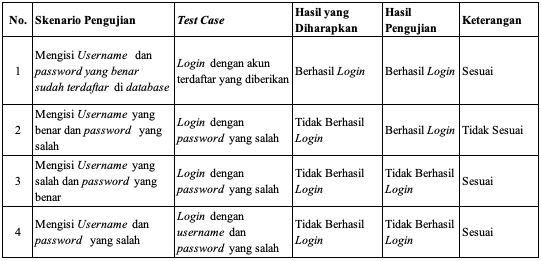
\includegraphics[width=12cm]{images/bab 4/fungsional-login.png}\\
                    \end{table}
                \item Pengujian Halaman \emph{Home}
                \begin{table}[ht]
                    \centering
                    \caption{Pengujian Halaman \emph{Home}}
                    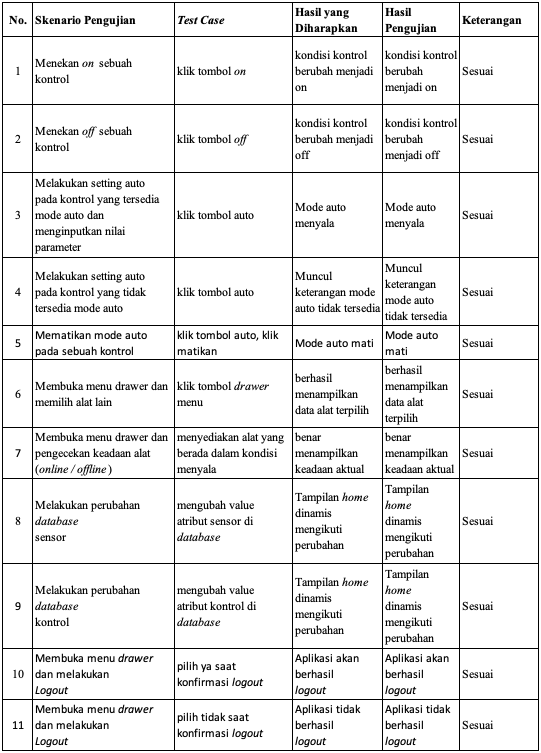
\includegraphics[width=11cm]{images/bab 4/fungsional-home.png}\\
                    \end{table}
            \end{itemize}
           
% \begin{table}[ht]
% \centering
% \caption{Permasalahan dan Solusinya}
% \begin{tabular}{|>{\raggedright}p{5cm}|p{2.5cm}|>{\raggedright}p{5cm}|}
%  \hline
%  \multicolumn{1}{|c}{\bfseries Masalah} & \multicolumn{1}{|c|}{\bfseries Aktor} & \multicolumn{1}{c|}{\bfseries Solusi} \\ 
%   \hline
% \begin{enumerate}
%    	\item Masalah masalah masalah Masalah masalah masalah Masalah masalah masalah Masalah masalah masalah.
%    	\item Masalah masalah masalah Masalah masalah masalah Masalah masalah masalah Masalah masalah masalah.
%    	\item Masalah masalah masalah Masalah masalah masalah Masalah masalah masalah Masalah masalah masalah.
%    \end{enumerate} &
%    \begin{enumerate}
%   	\item Aktor 1
%   	\item Aktor 2
%   \end{enumerate} &
%   \begin{enumerate}
%   \item Solusi solusi solusi Solusi solusi solusi Solusi solusi solusi Solusi solusi solusi Solusi solusi solusi.
%   \item Solusi solusi solusi Solusi solusi solusi Solusi solusi solusi Solusi solusi solusi Solusi solusi solusi.
%   \item Solusi solusi solusi Solusi solusi solusi Solusi solusi solusi Solusi solusi solusi Solusi solusi solusi.
%   \end{enumerate}
%      \tabularnewline
%   \hline
%  \end{tabular}
% \end{table}
        \vspace{1cm}
        \subsection{Uji Lapangan}
        Pada uji lapangan selain mengamati jalannya aplikasi sekaligus dilakukan pengujian UAT untuk mengetahui tingkat penerimaan pengguna dalam menggunakan aplikasi KEBUNQ.
        Setelah data kuesioner dikumpulkan kemudian dilakukan perhitungan persentase dengan cara mengalikan jumlah setiap pilihan jawaban 
        dengan 100 kemudian dibagi dengan jumlah responden. Persentase dapat dihitung dengan menggunakan rumus:
        \begin{equation}
            P = \frac{f}{n} \times 100\%
         \end{equation}
         \noindent Keterangan :
         \\P = Persentase
         \\n = Jumlah responden
         \\f = Frekuensi jawaban\\
         \begin{table}[ht]
            \centering
            \caption{Kuesioner}
            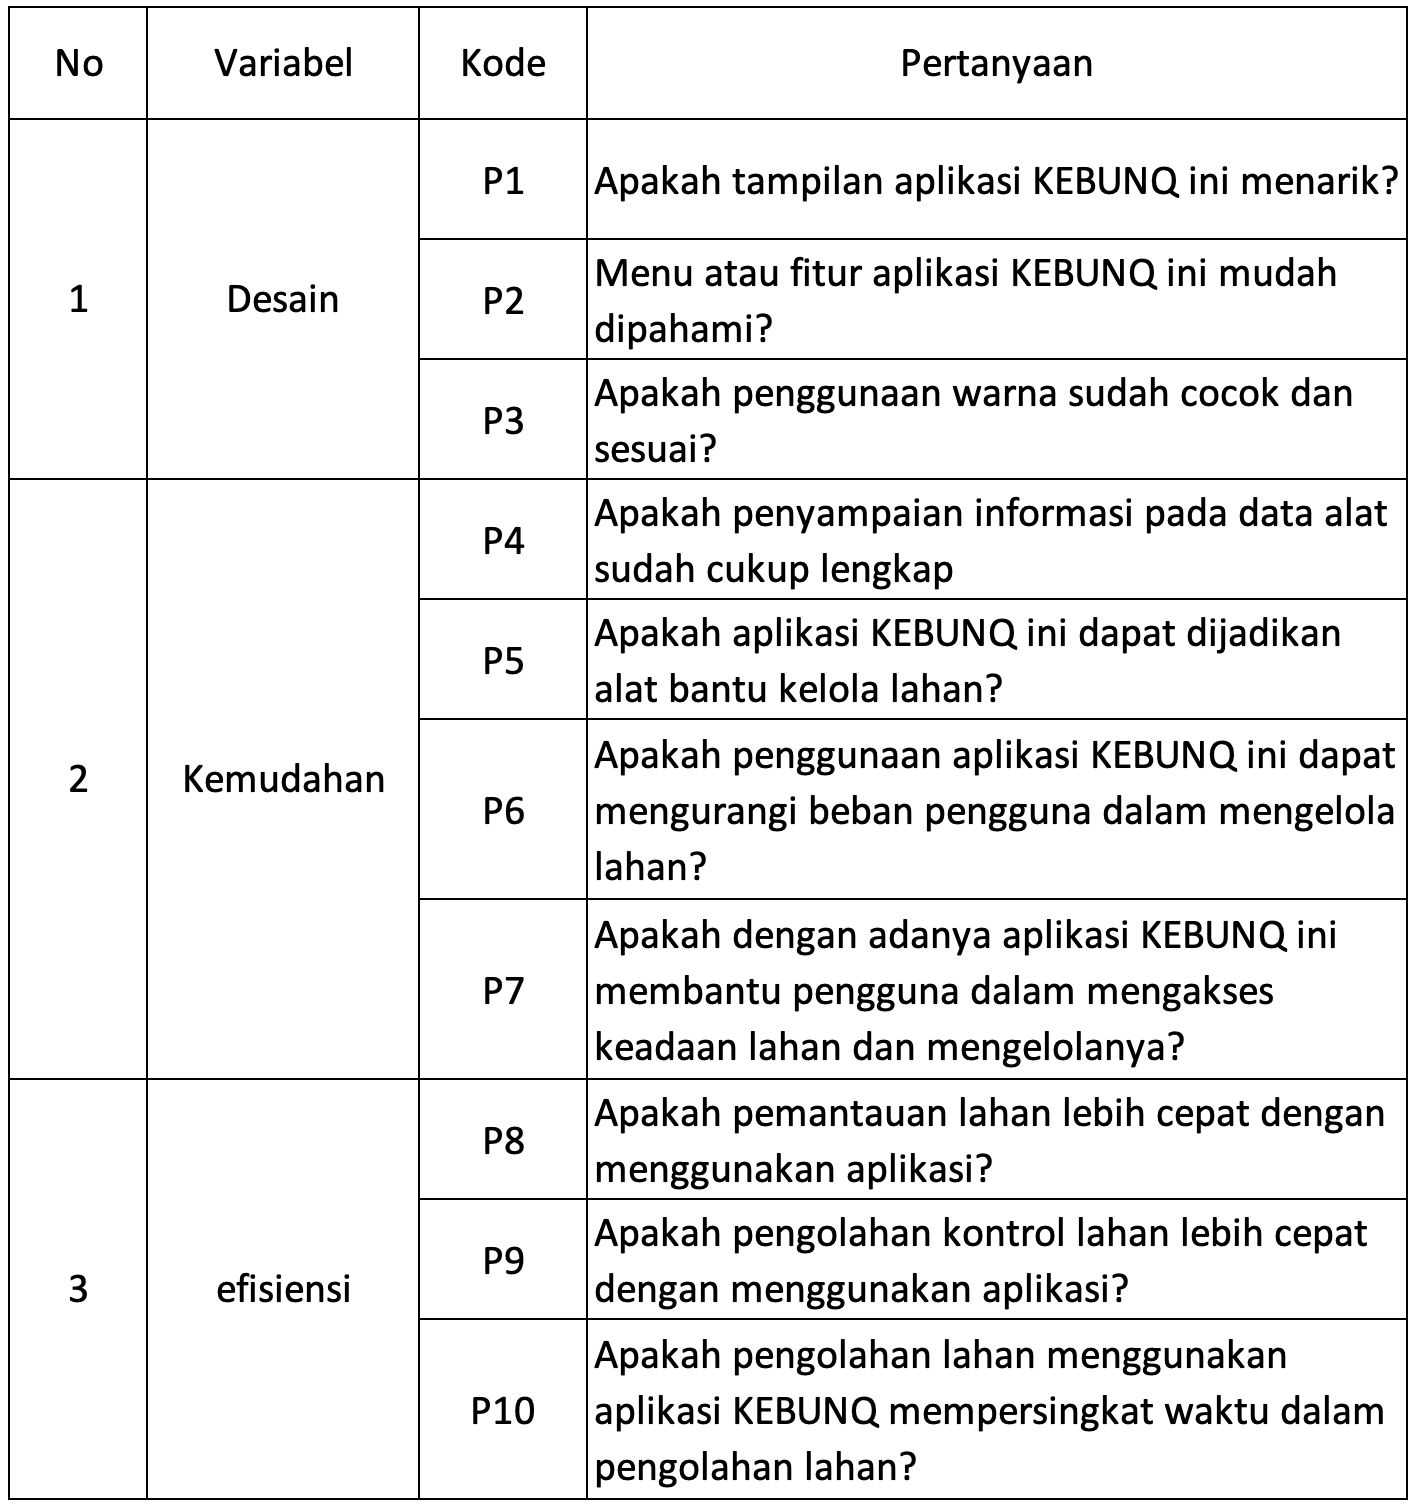
\includegraphics[width=11cm]{images/bab 4/uat.png}\\
            \end{table}
       \newline \noindent Hasil kuesioner yang dilakukan dijumlahkan berdasarkan setiap jawaban dapat dilihat pada tabel 4.4, berikut:\\
        \begin{table}[ht]
            \centering
            \caption{Kuesioner}
            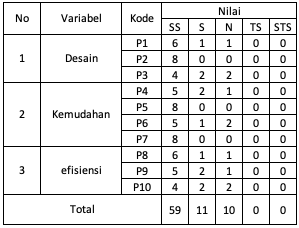
\includegraphics[width=8cm]{images/bab 4/hitungan.png}\\
            \end{table}
            \newline \noindent \\\\\\\\
            \vspace{5cm}
            \noindent \\Dari data tertera pada Tabel 4.4, dilakukan perhitungan dengan pemberian bobot pada total setiap jawaban.
            Perhitungan pembobotan dapat dilihat sebagai berikut:
            \begin{itemize}
                \item Jumlah skor responden Sangat Setuju (SS) = 59 x 5 = \textbf{295}
                \item Jumlah skor responden Setuju (S)  = 11 x 4 = \textbf{44}
                \item Jumlah skor responden Netral (N)  = 10 x 3 = \textbf{30}
                \item Jumlah skor responden Tidak Setuju (TS)  = 0 x 2 = \textbf{0}
                \item Jumlah skor responden Sangat Tidak Setuju (STS)  = 0 x 1 = \textbf{0}
            \end{itemize}
            Maka didapat jumlah total dari pemberian bobot adalah \textbf{369}\\
            Hasil jawaban dari 8 responden tersebut kemudian dilakukan perhitungan nilai terendah dan tertinggi seperti berikut:
            \begin{itemize}
                \item Nilai terendah = 8 x 10 x 1 = \textbf{80}
                \item Nilai tertinggi = 8 x 10 x 5 = \textbf{400}
             \end{itemize}
             Hasil perhitungan nilai tertinggi yang didapat adalah 400. Kemudian dilakukan perhitungan persentase menggunaan persamaan sebelumnya, sebagai berikut:
             \begin{equation}
                P = \frac{369}{400} \times 100\% = 92,2\%
             \end{equation}
             Berdasarkan perhitungan di atas, didapatkan bahwa tingkat penerimaan terhadap aplikasi KEBUNQ terletak pada rentang 81\% - 100\%, 
             masuk dalam kategori nilai kesimpulan sangat kuat sesuai dengan yang dikemukakan oleh Riduwan dalam referensi \cite{kuantitatif}, dengan nilai perhitungan persentase
             92,2\%, yang berarti aplikasi KEBUNQ ini dapat diterima oleh pengguna. Hasil persentase tersebut dapat dilihat pada skala penilaian pada Gambar 4.17 berikut ini:
             \begin{figure}[ht]
                \centering
                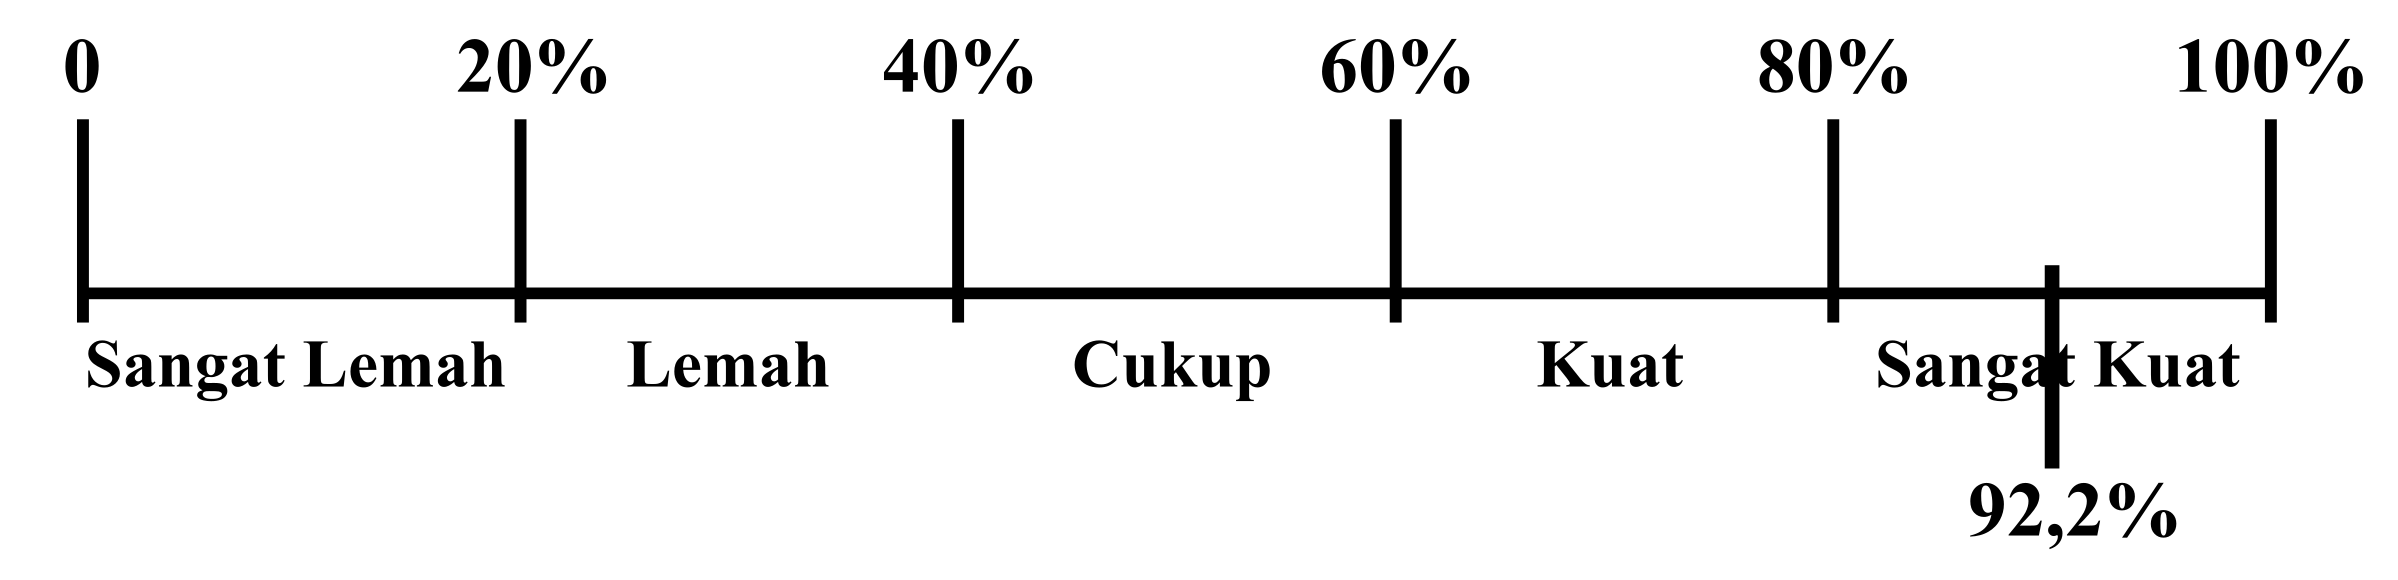
\includegraphics[width=8cm]{images/bab 4/persentase.png}
                \caption{Skala penilaian}
            \end{figure}


   
        \section{Pembahasan}
        Pada tahap observasi didapatkan jenis-jenis sensor dan kontrol yang akan dimasukkan pada penentuan bagaimana aplikasi dirancang dan dibuat. Pada tahap pembuatan aplikasi KEBUNQ, peneliti menggunakan \emph{framework Flutter} dengan bahasa pemrograman \emph{Dart}. Dalam penelitian ini dilakukan dua metode pengujian yaitu \emph{black box testing} dan UAT. Pada pengujian \emph{black box} terdapat satu hasil yang tidak sesuai dengan yang diharapkan, yaitu pada
        pengujian halaman login saat melakukan pengisian \emph{username} yang benar dan \emph{password} yang salah, setelah dilakukan pengecekan permasalahannya terdapat pada API login yang diterima peneliti 
        belum melakukan validasi password dan hanya melakukan validasi pada \emph{username}. Selanjutnya pada pengujian UAT, didapatkan hasil persentase sebesar 92,2\% yang menunjukkan penerimaan pengguna yang sangat kuat.
         

    








    \end{justify}




    
\end{flushleft}

\newpage
%-----------------------------------------------------------------------------%
\chapter{KESIMPULAN DAN SARAN}
%-----------------------------------------------------------------------------%

%
\vspace{4.5pt}

\begin{flushleft}
    \section{Kesimpulan}

    \section{Saran}
        
\end{flushleft}

\newpage

% Merubah Nama Bibliografi ke Daftar Pustaka
\renewcommand{\bibname}{DAFTAR PUSTAKA}
\phantomsection
\addcontentsline{toc}{chapter}{DAFTAR PUSTAKA}
% Daftar Pustaka

\begin{thebibliography}{7}
%\bibliographystyle{unsrt}
\providecommand{\natexlab}[1]{#1}
\providecommand{\url}[1]{\texttt{#1}}
\expandafter\ifx\csname urlstyle\endcsname\relax
  \providecommand{\doi}[1]{doi: #1}\else
  \providecommand{\doi}{doi: \begingroup \urlstyle{rm}\Url}\fi


\bibitem[1]{dokumenBalitbang}
BPTP Balitbangtan Jambi, "Alat dan Mesin Pertanian Tepat Guna untuk Tanaman Padidalam Mendukung Program Peningkatan Produksi Beras Nasional (P2BN)"
\newblock 2020, Available: http://jambi.litbang.pertanian.go.id/ind/images/PDF/Kiki1.pdf

\bibitem[2]{teknologi}
Admin dispmd, “Pengertian Teknologi Tepat Guna,” \emph{Dinas Pemberdayaan Masyarakat dan Desa}, 16-May-2018. [Online]. Available: https://dispmd.bulelengkab.go.id/informasi/detail/bank\_data/pengertian-teknologi-tepat-guna-13. [Accessed: 02-Feb-2022]. 

\bibitem[3]{web-datasmartphone}
Y. Pusparisa, “Daftar Negara Pengguna smartphone Terbanyak, Indonesia urutan berapa?: Databoks,” \emph{Databoks Pusat Data Ekonomi dan Bisnis Indonesia}, 01-Jul-2021. [Online]. Available: https://databoks.katadata.co.id/datapublish/2021/07/01/daftar-negara-pengguna-smartphone-terbanyak-indonesia-urutan-berapa. [Accessed: 06-Feb-2022]. 

\bibitem[4]{databps}
A. ID, “Jumlah Petani di indonesia - grafik alinea ID,” \emph{https://data.alinea.id/}, 11-Oct-2021. [Online]. Available: https://data.alinea.id/jumlah-petani-di-indonesia-b2cCd9Bp9c. [Accessed: 08-Feb-2022]. 

\bibitem[5]{jurnal-kajianAplikasi}
Direktorat Pangan dan Pertanian, “Studi Pendahuluan Rencana Pembangunan Jangka Menengah Nasional (RPJMN) Bidang Pangan dan Pertanian 2015 – 2016”, Direktorat Pangan dan Pertanian Kementerian Perancanaan Pembangunan Nasional/Badan Perencanaan Pembangunan Nasional, 2013.
% https://journal.uii.ac.id/Snati/article/download/6236/5598

\bibitem[6]{sdlc}
C. Jessica, “Software development life cycle (SDLC): Arti, Cara Kerja, Penerapan, Dan Manfaatnya,” \emph{Glints Blog}, 17-Dec-2021. [Online]. Available: https://glints.com/id/lowongan/sdlc-software-development-life-cycle/. [Accessed: 27-May-2022]. 

\bibitem[7]{sdlc2}
F. NKD, “Pengertian, model, Dan Tahapan SDLC\&nbsp; (software development life cycle),” \emph{Web developer LOGIQUE's Blog}, 28-Apr-2021. [Online]. Available: https://www.logique.co.id/blog/2021/04/28/tahapan-sdlc/. [Accessed: 27-May-2022]. 

\bibitem[8]{Sukamto}
Sukamto, R. A. dan Shalahudin, M.. Rekayasa Perangkat Lunak Terstruktur dan Berorientasi Objek. Bandung : Informatika Bandung, 2016.

\bibitem[9]{jurnal empiris}
P. Beynon-Davies, C. Carne, H. Mackay, and D. Tudhope, “Rapid application development (RAD): An empirical review,” \emph{European Journal of Information Systems}, vol. 8, no. 3, pp. 212, 1999. 
% https://www.researchgate.net/publication/31978101_Rapid_application_development_RAD_An_empirical_review

\bibitem[10]{web waterfall}
M. P. Putri and H. Effendi, “Implementasi metode RAD Pada website  service guide ‘Tour waterfall south sumatera’,” \emph{Jurnal Sisfokom (Sistem Informasi dan Komputer)}, vol. 7, no. 2, pp. 130–136, Sep. 2018. 
% https://www.google.com/url?sa=t&rct=j&q=&esrc=s&source=web&cd=&cad=rja&uact=8&ved=2ahUKEwjioNOUoeP3AhW88HMBHS9qCqkQFnoECAYQAQ&url=http%3A%2F%2Fjurnal.atmaluhur.ac.id%2Findex.php%2Fsisfokom%2Farticle%2Fview%2F00021&usg=AOvVaw2jJicE3WeLE5gyXS2aFEdB

\bibitem[11]{jurnal RAD UAT}
A. Rahman, "Rapid Application Development Sistem Pembelajaran Daring Berbasis Android," \emph{Jurnal Intech}, vol. 1, no. 2, pp. 20-25, Nov. 2020.
% https://www.google.com/url?sa=t&rct=j&q=&esrc=s&source=web&cd=&cad=rja&uact=8&ved=2ahUKEwitj6T-oOP3AhVS7XMBHf5rDaYQFnoECAYQAQ&url=https%3A%2F%2Fjournal.unbara.ac.id%2Findex.php%2FINTECH%2Farticle%2Fdownload%2F639%2F464%2F&usg=AOvVaw3MNPdSK6Bm-OYVrWqfrTL7

\bibitem[12]{jurnal RAD UAT 2}
D. Aryani, Malabay, H. D. Ariessanti, "Penerapan Rapid Application Development (RAD) Pada Perancangan Aplikasi Tracer Study Berbasis Android," \emph{eDikInformatika}, vol. 7, no. 1, pp. 111-122, Oct. 2020.
% https://digilib.esaunggul.ac.id/public/UEU-Journal-20259-11_1399.pdf

\bibitem[13]{Monitoring}
Hikmat, Dr. Harry. 2010. \emph{Monitoring dan Evaluasi Proyek}.

\bibitem[14]{Kontrol}
Katsuhiko Ogata. "Teknik kontrol automatik“, PT penerbit erlangga-SIMON. \&SCHUTER (ASUA) Pte.ltd., 1997.

\bibitem[15]{mobile}
N. Serrano, J. Hernantes and G. Gallardo. Mobile Web Apps. \emph{IEEE Software}, vol. 30, no. 5, 2013, pp. 22 -27.
% https://www.researchgate.net/publication/313868513_Studying_Mobile_Apps_for_Agriculture

\bibitem[16]{flutter}
Ganda, Yusmi P. W., Happy Flutter. Cetakan 1. Tangerang Selatan : Al Qolam, 2019.

\bibitem[17]{API}
IBM Cloud Education, “What is an application programming interface (API),” \emph{IBM}, 19-Aug-2020. [Online]. Available: https://www.ibm.com/cloud/learn/api. [Accessed: 11-Feb-2022]. 

\bibitem[18]{Database}
OCI, “What is a database?,” \emph{Oracle}, 2022. [Online]. Available: https://www.oracle.com/database/what-is-database/. [Accessed: 11-Feb-2022]. 

\bibitem[19]{Flowchart}
“What is a flowchart?,” \emph{ASQ}. [Online]. Available: https://asq.org/quality-resources/flowchart. [Accessed: 15-Feb-2022]. 

\bibitem[20]{gambar fc}
D. Rizky, “Jenis Flowchart Dan Simbol-Simbolnya,” \emph{Medium}, 30-Apr-2019. [Online]. Available: https://medium.com/dot-intern/jenis-flowchart-dan-simbol-simbolnya-ef6553c53d73. [Accessed: 20-Feb-2022]. 

\bibitem[21]{use case 1}
M. R. Adani, “Use case diagram: Pengertian, Fungsi, Teknik, Dan Contoh,” \emph{Sekawan Media | Software House \&amp; System Integrator Indonesia}, 21-Jun-2021. [Online]. Available: https://www.sekawanmedia.co.id/blog/use-case-diagram/. [Accessed: 20-Feb-2022]. 

\bibitem[22]{use case 2}
Lucid Software, “UML use case diagram tutorial,” \emph{Lucidchart}. [Online]. Available: https://www.lucidchart.com/pages/uml-use-case-diagram. [Accessed: 24-Feb-2022]. 

\bibitem[23]{figma uc}
F. Mandrelli, “UML use case diagram,” \emph{Figma}, 2021. [Online]. Available: https://www.figma.com/community/file/986330591099819762. [Accessed: 24-Feb-2022]. 

\bibitem[24]{buku scholar}
R.   Habibi   and   R.   Aprilian,   Tutorial   dan Penjelasan  Aplikasi  E-Office  Berbasis  Web Menggunakan Metode RAD, Bandung: Kreatif Industri Nusantara, 2020. 
% bukunya https://books.google.co.id/books?hl=id&lr=&id=h5PuDwAAQBAJ&oi=fnd&pg=PR1&dq=related:MMIDeyjXtEUJ:scholar.google.com/&ots=Ht-Xb71R5S&sig=X1LON_cyff00KLfgqs0woyCpU-Q&redir_esc=y#v=onepage&q&f=false
% akun beliau https://scholar.google.co.id/citations?view_op=view_citation&hl=id&user=IBtTXDAAAAAJ&citation_for_view=IBtTXDAAAAAJ:LkGwnXOMwfcC
%  halaman 101

\bibitem[25]{black box}
Iskandaria. 2012. Contoh Pengujian Black Box

\bibitem[26]{uat}
Mutiara, A. B., Awaludin, R., Muslim, A. and T. Oswari, “Testing Implementasi Website Rekam Medis Elektronik Opeltgunasys Dengan Metode Acceptance Testing,” 2014.

\bibitem[27]{likert}
Sugiyono, \emph{Memahami Penelitian Kualitatif}. Bandung, Indonesia: Alfabeta, 2012.

\bibitem[28]{kuantitatif}
Riduwan, \emph{Belajar mudah penelitian untuk guru-karyawan dan peneliti pemula}. Bandung, Indonesia: Alfabeta, 2009. 


\end{thebibliography}



%
% Lampiran 
%

\setcounter{originalpagenumber}{\number\value{page}}%
\setcounter{page}{0}
\pagenumbering{arabic}

\onehalfspacing
\begin{appendix}
	%
% @author  Andreas Febrian
% @version 1.00 
% 
% Hanya sebuah pembatas bertuliskan LAMPIRAN ditengah halaman. 
% 

\begin{titlepage}
	\centering 
	\vspace*{6cm}
	\noindent \Huge{LAMPIRAN}
\end{titlepage}
\end{appendix}

\pagenumbering{arabic}% 
\setcounter{page}{\number\value{originalpagenumber}}
\clearpage
\phantomsection \addcontentsline{toc}{chapter}{LAMPIRAN}

%-----------------------------------------------------------------------------%
\section*{Coding Login Aplikasi}
%-----------------------------------------------------------------------------%



\end{document}